\documentclass[11pt]{amsart}
\usepackage[utf8]{inputenc}
\usepackage{graphicx}
\usepackage{amssymb}
\usepackage{amsmath}
\usepackage{booktabs}
\usepackage{listings}
\usepackage[margin=2.8cm]{geometry}
\usepackage[hidelinks]{hyperref}

\graphicspath{{figures/}}

\newcommand{\R}{\mathbb R}
\newcommand{\N}{\mathbb{N}}
\newcommand{\LL}{\mathcal L}
\newcommand{\T}{\mathcal T}
\newcommand{\dx}{\,dx}
\newcommand{\pp}{p(\cdot)}
\DeclareMathOperator{\dvg}{div}

\newtheorem{teo}{Theorem}[section]
\newtheorem{lema}[teo]{Lemma}
\newtheorem{prop}[teo]{Proposition}
\newtheorem{corol}[teo]{Corollary}
\theoremstyle{definition}
\newtheorem{defi}[teo]{Definition}
\newtheorem{question}[teo]{Open question}
\theoremstyle{remark}
\newtheorem{remark}[teo]{Remark}

\numberwithin{equation}{section}

\lstset{basicstyle=\ttfamily\small, columns=fullflexible, keepspaces=true,
  frame=single, framerule=0.3pt, xleftmargin=1em, xrightmargin=1em, language=Python,
  showstringspaces=false, commentstyle=\itshape}

\title[Numerical computation of \texorpdfstring{$p(x)$}{p(x)}-Laplace equations]{Effective numerical computation of $p(x)$-Laplace equations on general planar domains}

\author[A. Arag\'on, J. Fern\'andez Bonder and D. Rubio]
{Adriana Arag\'on, Juli\'an Fern\'andez Bonder and Diana Rubio}

\address{Adriana Arag\'on and Diana Rubio \hfill\break\indent
Centro de Matem\'atica Aplicada (CEDEMA), Universidad Nacional de San Mart\'in,
Tornav\'ias Mart\'in de Irigoyen No.3100, Campus Miguelete, B1650 Villa Lynch, Provincia de Buenos Aires, Argentina.}

\email[A. Arag\'on]{\tt aaragon@unsam.edu.ar}
\email[D. Rubio]{\tt drubio@unsam.edu.ar}

\address{Juli\'an Fern\'andez Bonder \hfill\break\indent
Departamento  de Matem\'atica, FCEN -- Universidad de Buenos Aires, and\hfill\break\indent
Instituto de C\'alculo -- CONICET\hfill\break\indent $0+\infty$ building, Ciudad Universitaria (1428), Buenos Aires, Argentina.}

\email{{\tt jfbonder@dm.uba.ar}\hfill\break\indent {\it Web page:} {\tt http://mate.dm.uba.ar/$\sim$jfbonder}}

\thanks{This is a modified version of the article \emph{Effective numerical computation of $p(x)$-Laplace equations in 2D} by the same authors, updated with a new implementation and new numerical experiments}
\thanks{JFB is supported by CONICET PIP N\textsuperscript{o} 11220150100032CO and by ANPCyT, PICT 2016-1022 and is a member of CONICET}

\subjclass[2020]{65N30, 35J92, 65K10}

\keywords{$p(x)$-Laplacian, variable exponent, finite elements, decomposition--coordination method, augmented Lagrangian}

\begin{document}

\begin{abstract}
We study the numerical solution of the Dirichlet problem for the $p(x)$-Laplacian, $-\dvg(|\nabla u|^{p(x)-2}\nabla u)=f$, on bounded planar domains by the decomposition--coordination method combined with piecewise linear finite elements. The method is derived from the optimality conditions of an augmented Lagrangian; each iteration consists of the solution of a linear Poisson-type problem, whose matrix does not change during the iteration, and of a pointwise nonlinear equation that reduces to a scalar equation with a unique root in an explicit interval. We recall the convergence result available for $p(x)\ge 2$ and describe a vectorised Python implementation that works on arbitrary triangulated planar domains (rectangles, polygons with holes, domains given by signed distance functions, imported meshes). The experiments include the standard test problems with explicit solutions, the observed order of convergence for the $p$-torsion problem on the disk as a function of $p$, the behaviour of the iteration as $p\to 1$, variable exponents (including a discontinuous one) with explicit solutions, and examples on non-rectangular domains.
\end{abstract}

\maketitle

%=====================================================================
\section{Introduction}
%=====================================================================

In this article we consider nonlinear elliptic problems with nonstandard growth driven by the $p(x)$-Laplace operator
$$
\Delta_{p(x)} u = \dvg\left( |\nabla u|^{p(x)-2}\nabla u\right).
$$
This operator appears in several applications, for instance in models of electrorheological fluids and in image processing; see \cite{CLR, R} and the references therein. When $p(x)\equiv p$ is constant it reduces to the $p$-Laplacian, which has been studied extensively from both the theoretical and the computational point of view; see, e.g., \cite{BL}. When $p$ is not constant the operator is no longer homogeneous, and the natural functional framework is that of Lebesgue and Sobolev spaces with variable exponent \cite{DHHR}.

We are concerned with the Dirichlet problem
\begin{equation}\label{eq.1}
\begin{cases}
-\Delta_{p(x)} u = f & \text{ in }\Omega,\\
u=g & \text{ on }\partial\Omega.
\end{cases}
\end{equation}
Throughout the paper we assume:
\begin{itemize}
\item[(A1)] $\Omega\subset\R^2$ is a bounded Lipschitz domain;
\item[(A2)] $p\colon\Omega\to\R$ is measurable and $1<p^-\le p(x)\le p^+<\infty$ for a.e.\ $x\in\Omega$, where $p^-=\operatorname{ess\,inf}_\Omega p$ and $p^+=\operatorname{ess\,sup}_\Omega p$;
\item[(A3)] $f\in L^2(\Omega)$, and $g$ is the trace of a function $\tilde g\in H^1(\Omega)$ with $|\nabla \tilde g|\in L^{\pp}(\Omega)$.
\end{itemize}
Continuity of $p$ is not required by the method, and some of the experiments below use discontinuous exponents.

The computation of solutions of \eqref{eq.1} is made difficult by the strong nonlinearity and by the degenerate ($p(x)>2$) or singular ($p(x)<2$) character of the operator at points where $\nabla u=0$. Among the first rigorous analyses of numerical approximations of \eqref{eq.1} is \cite{DPLM}, where an interior penalty discontinuous Galerkin method is studied; see also \cite{D} for a finite element analysis of a related model of electrorheological fluids and \cite{DPM2} for orders of convergence of the finite element method. A different approach, based on a quasi-Newton minimisation of the energy functional that takes the singular/degenerate behaviour into account, is developed in \cite{CZ}.

In \cite{DPM} the \emph{decomposition--coordination method} was applied to problem \eqref{eq.1}. This method goes back to Glowinski and Marrocco \cite{GM} and Gabay and Mercier \cite{GaM} (see also \cite{FG, Glowinski}); it is nowadays also known as the alternating direction method of multipliers (ADMM) \cite{Boyd}. It is an iterative procedure in which each step requires the solution of a \emph{linear} elliptic problem, always with the same operator, and of a \emph{nonlinear algebraic} equation that decouples pointwise. In the present paper we
\begin{enumerate}
\item derive the iteration, for a general augmented Lagrangian parameter $r>0$, from the optimality conditions of the augmented Lagrangian, and analyse the pointwise equation (Section~\ref{sec.method});
\item recall the convergence result that follows from \cite{Glowinski} when $p(x)\ge2$, and formulate the case $1<p(x)<2$ as an open question (Section~\ref{sec.convergence});
\item describe a discretisation by piecewise linear finite elements and a vectorised Python implementation, valid for arbitrary triangulations of planar domains and publicly available (Section~\ref{sec.implementation});
\item report numerical experiments (Section~\ref{sec.experiments}): the classical test problems, the observed order of convergence for the $p$-torsion problem on the disk as a function of $p$, the behaviour of the iteration as $p\to1$, variable exponents with explicit solutions, and non-rectangular domains.
\end{enumerate}
Section~\ref{sec.conclusions} summarises the conclusions and the limitations of the study.

%=====================================================================
\section{The decomposition--coordination method}\label{sec.method}
%=====================================================================

\subsection{Notation}
For a measurable function $w$ on $\Omega$, scalar or vector valued, we denote by
$$
J_{p}(w) := \int_\Omega |w(x)|^{p(x)}\dx\in[0,\infty]
$$
the $p(\cdot)$-\emph{modular} of $w$. The variable exponent Lebesgue space $L^{\pp}(\Omega)$ is the set of measurable $w$ with $J_p(w)<\infty$ (under (A2) this is equivalent to $J_p(\lambda w)<\infty$ for all $\lambda>0$), endowed with the Luxemburg norm
$$
\|w\|_{L^{\pp}(\Omega)} := \inf\{\lambda>0\colon J_p(w/\lambda)\le 1\}.
$$
If $J_p(w)\le 1$, then $\|w\|_{L^{\pp}(\Omega)}^{p^+}\le J_p(w)\le\|w\|_{L^{\pp}(\Omega)}^{p^-}$; see \cite[Chapter~2]{DHHR}. In particular $J_p(w)^{1/p^+}$ is an upper bound for the Luxemburg norm when $J_p(w)\le1$, and for constant $p$ it coincides with the $L^p$ norm. This motivates the quantity
\begin{equation}\label{eq.pnorm}
\mathcal M_p(w) := J_p(w)^{1/p^+},
\end{equation}
which is used below as a stopping quantity and, for comparison purposes, to measure errors. We stress that $\mathcal M_p$ is not a norm when $p$ is not constant: it is not homogeneous, and for small $w$ it behaves like a power $p^-/p^+<1$ of a norm, so that it can be much larger than, e.g., the maximum norm of $w$. $W^{1,\pp}(\Omega)$ is the space of $w\in L^{\pp}(\Omega)$ with $|\nabla w|\in L^{\pp}(\Omega)$, and $W^{1,\pp}_0(\Omega)$ denotes the closure of $C^\infty_c(\Omega)$ in it. Under (A2) these spaces are reflexive Banach spaces \cite{DHHR}. Since $p^->1$ and $\Omega\subset\R^2$ is bounded, $W^{1,\pp}_0(\Omega)\subset W^{1,p^-}_0(\Omega)\hookrightarrow L^2(\Omega)$ by the Sobolev embedding, so $f\in L^2(\Omega)$ defines a continuous linear functional on $W^{1,\pp}_0(\Omega)$.

A \emph{weak solution} of \eqref{eq.1} is a function $u\in\tilde g+W^{1,\pp}_0(\Omega)$ such that
\begin{equation}\label{eq.weak}
\int_\Omega |\nabla u|^{p(x)-2}\nabla u\cdot\nabla w\dx=\int_\Omega fw\dx\qquad\text{for all } w\in W^{1,\pp}_0(\Omega).
\end{equation}
Equivalently, $u$ is the minimiser in $\tilde g+W^{1,\pp}_0(\Omega)$ of the strictly convex and coercive energy
\begin{equation}\label{eq.energy}
E(v) = \int_\Omega \frac{|\nabla v|^{p(x)}}{p(x)}\dx-\int_\Omega fv\dx ,
\end{equation}
whose existence and uniqueness follow from the direct method of the calculus of variations. Here and below, for $\xi\in\R^2$ and $p>1$, the vector $|\xi|^{p-2}\xi$ is understood to be $0$ when $\xi=0$; the map $\xi\mapsto|\xi|^{p-2}\xi$ is continuous on $\R^2$ and is the gradient of the convex $C^1$ function $\xi\mapsto|\xi|^p/p$.

\subsection{Augmented Lagrangian and the algorithm}
Write $H:=L^2(\Omega)^2$, with inner product $(\cdot,\cdot)$ and norm $\|\cdot\|$, and $V_g:=\tilde g+H^1_0(\Omega)$. Define
$$
F(q):=\int_\Omega\frac{|q|^{p(x)}}{p(x)}\dx\in[0,\infty]\quad(q\in H),\qquad G(v):=-\int_\Omega fv\dx\quad(v\in H^1(\Omega)).
$$
The problem $\min_v F(\nabla v)+G(v)$ is rewritten as the constrained problem of minimising $F(q)+G(v)$ subject to $\nabla v=q$. For $r>0$ the corresponding \emph{augmented Lagrangian} is
\begin{equation}\label{eq.Lr}
\LL_r(v,q,\mu) := F(q)+G(v)+(\mu,\nabla v-q)+\frac r2\|\nabla v-q\|^2,\qquad (v,q,\mu)\in V_g\times H\times H,
\end{equation}
with values in $(-\infty,+\infty]$. The decomposition--coordination method (algorithm ALG2 in \cite{FG, Glowinski}, with multiplier step equal to $r$) minimises $\LL_r$ alternately in $v$ and in $q$ and then updates the multiplier:

\medskip
\noindent\textbf{Algorithm DC($r$).} Choose $\nu_0\in H$ with $F(\nu_0)<\infty$ and $\eta_1\in H$ (in practice $\nu_0=\eta_1=0$). For $n=1,2,\dots$:
\begin{enumerate}
\item[(i)] compute $u_n\in V_g$ such that
\begin{equation}\label{eq.u}
r\int_\Omega\nabla u_n\cdot\nabla w\dx=\int_\Omega fw\dx+\int_\Omega(r\nu_{n-1}-\eta_n)\cdot\nabla w\dx\qquad\text{for all }w\in H^1_0(\Omega),
\end{equation}
that is, $-r\Delta u_n=f+\dvg(\eta_n-r\nu_{n-1})$ in $\Omega$, $u_n=g$ on $\partial\Omega$;
\item[(ii)] compute $\nu_n\in H$ such that, for a.e.\ $x\in\Omega$,
\begin{equation}\label{eq.nu}
|\nu_n|^{p(x)-2}\nu_n+r\nu_n=\eta_n+r\nabla u_n;
\end{equation}
\item[(iii)] update the multiplier
\begin{equation}\label{eq.eta}
\eta_{n+1}=\eta_n+r(\nabla u_n-\nu_n).
\end{equation}
\end{enumerate}

The default value used throughout the paper is $r=1$, for which the steps read
$$
-\Delta u_n=f+\dvg(\eta_n-\nu_{n-1}),\qquad |\nu_n|^{p(x)-2}\nu_n+\nu_n=\eta_n+\nabla u_n,\qquad \eta_{n+1}=\eta_n+\nabla u_n-\nu_n.
$$
We use $\nu$ for the auxiliary (algebraic) unknown, which approximates $\nabla u$, and $\eta$ for the multiplier, which approximates the flux $|\nabla u|^{p(x)-2}\nabla u$ (see Lemma~\ref{lem.saddle}). Note the sign in \eqref{eq.u}: the right-hand side of the weak form is $\int f w+\int(r\nu_{n-1}-\eta_n)\cdot\nabla w$.

\subsection{The pointwise equation}
The next lemma deals with the nonlinear step \eqref{eq.nu}, which decouples in $x$.

\begin{lema}\label{lem.scalar}
Let $p>1$ and $r>0$.
\begin{enumerate}
\item[(a)] For every $s\ge0$ the equation
\begin{equation}\label{eq.scalar}
t^{p-1}+rt=s,\qquad t\ge0,
\end{equation}
has a unique solution $t=t(p,s)$. It satisfies $t(p,0)=0$ and
\begin{equation}\label{eq.bracket}
\min\Big\{\frac{s}{2r},\Big(\frac s2\Big)^{\frac1{p-1}}\Big\}\le t(p,s)\le\min\Big\{\frac sr,\ s^{\frac1{p-1}}\Big\}.
\end{equation}
The map $(p,s)\mapsto t(p,s)$ is continuous on $(1,\infty)\times[0,\infty)$.
\item[(b)] For every $w\in\R^2$ the equation $|\nu|^{p-2}\nu+r\nu=rw$ has the unique solution
\begin{equation}\label{eq.nu.formula}
\nu=\Phi_r(p,w):=\begin{cases}\dfrac{t(p,r|w|)}{|w|}\,w,& w\neq0,\\[2mm] 0,& w=0,\end{cases}
\end{equation}
and $|\Phi_r(p,w)|\le|w|$. The map $\Phi_r$ is continuous on $(1,\infty)\times\R^2$.
\item[(c)] For every $w\in\R^2$, $\Phi_r(p,w)$ is the unique minimiser of the strictly convex function
$\varphi(\xi)=\frac1p|\xi|^p+\frac r2|\xi|^2-r\,w\cdot\xi$ on $\R^2$.
\end{enumerate}
\end{lema}

\begin{proof}
(a) The function $\psi(t)=t^{p-1}+rt$ is continuous and strictly increasing on $[0,\infty)$, with $\psi(0)=0$ and $\psi(t)\to\infty$ as $t\to\infty$; hence \eqref{eq.scalar} has exactly one solution, and $t(p,0)=0$. Since both terms of $\psi$ are nonnegative, $rt\le s$ and $t^{p-1}\le s$, which is the upper bound in \eqref{eq.bracket}. Since $\psi(t)=s$, at least one of the two terms is $\ge s/2$, i.e.\ $t\ge s/(2r)$ or $t\ge (s/2)^{1/(p-1)}$, which gives the lower bound. For continuity, let $(p_k,s_k)\to(p,s)$ with $p>1$ and set $t_k=t(p_k,s_k)$. By the upper bound, $(t_k)$ is bounded; if $t_{k_j}\to\tau$ along a subsequence, passing to the limit in $t_{k_j}^{p_{k_j}-1}+rt_{k_j}=s_{k_j}$ gives $\psi(\tau)=s$ (note that $t^{q}\to\tau^{p-1}$ as $t\to\tau$, $q\to p-1>0$, also when $\tau=0$), so $\tau=t(p,s)$ by uniqueness. Hence the whole sequence converges to $t(p,s)$.

(b) Let $A(\xi)=|\xi|^{p-2}\xi+r\xi$. For $\xi,\zeta\in\R^2$, $(A(\xi)-A(\zeta))\cdot(\xi-\zeta)\ge r|\xi-\zeta|^2$, because $\xi\mapsto|\xi|^{p-2}\xi$ is the gradient of a convex function and therefore monotone. Thus $A$ is injective and the equation $A(\nu)=rw$ has at most one solution. If $w=0$, $\nu=0$ is a solution. If $w\ne0$, put $t=t(p,r|w|)$ and $\nu=(t/|w|)w$; then $|\nu|=t$ and
$t>0$ (because $\psi(t)=r|w|>0=\psi(0)$) and
$A(\nu)=(t^{p-2}+r)\,t\,\frac{w}{|w|}=\psi(t)\frac{w}{|w|}=r|w|\frac{w}{|w|}=rw$. The bound $|\nu|=t\le r|w|/r=|w|$ follows from \eqref{eq.bracket}. Continuity of $\Phi_r$ at points with $w\ne0$ follows from (a); at $w=0$ it follows from $|\Phi_r(p,w)|\le|w|$.

(c) $\varphi$ is $C^1$, strictly convex (it is the sum of a convex and a strictly convex function) and coercive, so it has a unique minimiser, characterised by $\nabla\varphi(\xi)=A(\xi)-rw=0$. By (b), this point is $\Phi_r(p,w)$.
\end{proof}

\begin{remark}\label{rem.bisection}
By \eqref{eq.bracket} the root of \eqref{eq.scalar} lies in the explicit interval $[0,\min\{s/r,s^{1/(p-1)}\}]$, so it can be computed by bisection without any safeguard; $k$ bisection steps produce an interval of length $2^{-k}\min\{s/r,s^{1/(p-1)}\}$ containing the root. The lower bound in \eqref{eq.bracket} shows that after $k$ steps the relative error is at most $2^{-k}\max\{2,2^{1/(p-1)}\}$, a pessimistic bound when $p$ is close to $1$. Computing $\nu$ through \eqref{eq.nu.formula} avoids evaluating $|\nu|^{p-2}$, which is singular at $\nu=0$ when $p<2$.
\end{remark}

\subsection{Derivation of the algorithm}
The following proposition shows that Algorithm DC($r$) is well defined and that its steps are exactly the alternating minimisation of $\LL_r$ followed by a multiplier update.

\begin{prop}\label{prop.derivation}
Assume (A1)--(A3), let $r>0$, $\nu_{n-1}\in H$ with $F(\nu_{n-1})<\infty$, and $\eta_n\in H$. Then:
\begin{enumerate}
\item[(a)] Problem \eqref{eq.u} has a unique solution $u_n\in V_g$, which is the unique minimiser over $V_g$ of $v\mapsto\LL_r(v,\nu_{n-1},\eta_n)$.
\item[(b)] The function $\nu_n(x):=\Phi_r\big(p(x),\eta_n(x)/r+\nabla u_n(x)\big)$ is the unique solution of \eqref{eq.nu} in $H$; it satisfies $F(\nu_n)<\infty$, and it is the unique minimiser over $H$ of $q\mapsto\LL_r(u_n,q,\eta_n)$.
\item[(c)] The updated multiplier is the flux associated with $\nu_n$: $\eta_{n+1}=|\nu_n|^{p(x)-2}\nu_n$ a.e.
\item[(d)] Consequently the sequence $(u_n,\nu_n,\eta_{n+1})$ generated by Algorithm DC($r$) is well defined, and it coincides with the sequence generated by
\begin{equation}\label{eq.alg2}
u_n=\operatorname*{argmin}_{v\in V_g}\LL_r(v,\nu_{n-1},\eta_n),\qquad
\nu_n=\operatorname*{argmin}_{q\in H}\LL_r(u_n,q,\eta_n),\qquad
\eta_{n+1}=\eta_n+r(\nabla u_n-\nu_n).
\end{equation}
\end{enumerate}
\end{prop}

\begin{proof}
(a) Since $F(\nu_{n-1})<\infty$, for $v\in V_g$
$$
\LL_r(v,\nu_{n-1},\eta_n)=F(\nu_{n-1})-(\eta_n,\nu_{n-1})+\Big[-\int_\Omega fv\dx+(\eta_n,\nabla v)+\frac r2\|\nabla v-\nu_{n-1}\|^2\Big]
$$
is finite, and only the bracket depends on $v$. Writing $v=\tilde g+z$ with $z\in H^1_0(\Omega)$, the bracket is a continuous quadratic functional of $z$ whose quadratic part is $\frac r2\|\nabla z\|^2$, which is coercive on $H^1_0(\Omega)$ by the Poincar\'e inequality. Hence it has a unique minimiser, characterised by the vanishing of its derivative in every direction $w\in H^1_0(\Omega)$:
$$
-\int_\Omega fw\dx+(\eta_n,\nabla w)+r(\nabla v-\nu_{n-1},\nabla w)=0\qquad\text{for all }w\in H^1_0(\Omega),
$$
which is exactly \eqref{eq.u}. (Equivalently, \eqref{eq.u} has a unique solution by the Lax--Milgram lemma.)

(b) Put $w_n=\eta_n/r+\nabla u_n\in H$. By Lemma~\ref{lem.scalar}(b), $\nu_n(x)$ solves \eqref{eq.nu} for every $x$, and it is the only solution of \eqref{eq.nu} at every $x$. It is measurable, as the composition of the continuous map $\Phi_r$ with the measurable map $x\mapsto(p(x),w_n(x))$, and $|\nu_n|\le|w_n|$, so $\nu_n\in H$. Moreover $F(\nu_n)<\infty$: where $|\nu_n|\le1$ we have $|\nu_n|^{p(x)}\le1$, and where $|\nu_n|>1$ and $p(x)\le 2$ we have $|\nu_n|^{p(x)}\le|w_n|^2$; where $|\nu_n|>1$ and $p(x)>2$ we use \eqref{eq.nu}: $|\nu_n|^{p(x)-1}\le |\eta_n+r\nabla u_n|=r|w_n|$, hence $|\nu_n|^{p(x)}\le (r|w_n|)^{p(x)/(p(x)-1)}\le \max\{1,r|w_n|\}^{2}$, which is integrable.

For $q\in H$ we have
$$
\LL_r(u_n,q,\eta_n)=G(u_n)+(\eta_n,\nabla u_n)+\frac r2\|\nabla u_n\|^2+\int_\Omega\varphi_x(q(x))\dx,
$$
where $\varphi_x(\xi)=\frac1{p(x)}|\xi|^{p(x)}+\frac r2|\xi|^2-r\,w_n(x)\cdot\xi$, and the integral takes values in $(-\infty,+\infty]$ because the negative part of $\varphi_x(q(x))$ is bounded by $r|w_n||q|\in L^1$. By Lemma~\ref{lem.scalar}(c), $\varphi_x(\nu_n(x))\le\varphi_x(q(x))$ for a.e.\ $x$, with strict inequality wherever $q(x)\ne\nu_n(x)$. Since $\int\varphi_x(\nu_n)\dx$ is finite, $\nu_n$ minimises $q\mapsto\LL_r(u_n,q,\eta_n)$, and any other minimiser must coincide with $\nu_n$ a.e.

(c) By \eqref{eq.nu} and \eqref{eq.eta}, $\eta_{n+1}=\eta_n+r\nabla u_n-r\nu_n=|\nu_n|^{p(x)-2}\nu_n$.

(d) By (b), $F(\nu_n)<\infty$, so (a) can be applied at the next step. The claim follows by induction from (a) and (b), starting from $F(\nu_0)<\infty$.
\end{proof}

\begin{remark}[Nonhomogeneous boundary data]\label{rem.lift}
Writing $u=\tilde g+z$ and $\nu=\nabla\tilde g+q$ with $z\in H^1_0(\Omega)$, one has $\nabla u-\nu=\nabla z-q$, so that $\LL_r(u,\nu,\eta)=\tilde F(q)+G(z)+(\eta,\nabla z-q)+\frac r2\|\nabla z-q\|^2+G(\tilde g)$ with $\tilde F(q):=F(q+\nabla\tilde g)$. Thus Algorithm DC($r$) with data $g$ is Algorithm ALG2 for the convex, proper, lower semicontinuous functional $\tilde F$ on the linear space $H^1_0(\Omega)\times H$, and in the convergence analysis we may assume $g=0$ without loss of generality.
\end{remark}

%=====================================================================
\section{Convergence}\label{sec.convergence}
%=====================================================================

We take $g=0$ (see Remark~\ref{rem.lift}) and write $V=H^1_0(\Omega)$. A triple $(u^*,\nu^*,\eta^*)\in V\times H\times H$ is a \emph{saddle point} of $\LL_r$ if
$$
\LL_r(u^*,\nu^*,\eta)\le\LL_r(u^*,\nu^*,\eta^*)\le\LL_r(v,q,\eta^*)\qquad\text{for all }(v,q,\eta)\in V\times H\times H.
$$
Since $\LL_r(0,0,\eta^*)=0$, the value $\LL_r(u^*,\nu^*,\eta^*)$ at a saddle point is finite. The saddle points have the following explicit description.

\begin{lema}\label{lem.saddle}
Assume (A1)--(A3) with $g=0$ and let $r>0$. A triple $(u^*,\nu^*,\eta^*)\in V\times H\times H$ is a saddle point of $\LL_r$ if and only if
\begin{equation}\label{eq.saddle}
\begin{gathered}
\nu^*=\nabla u^*,\qquad F(\nu^*)<\infty,\qquad \eta^*=|\nabla u^*|^{p(x)-2}\nabla u^*\ \text{ a.e. in }\Omega,\\
(\eta^*,\nabla w)=\int_\Omega fw\dx\quad \text{ for all } w\in V.
\end{gathered}
\end{equation}
In that case $u^*$ minimises $v\mapsto F(\nabla v)+G(v)$ over $V$, and the saddle points of $\LL_r$ do not depend on $r$.
\end{lema}

\begin{proof}
Let $(u^*,\nu^*,\eta^*)$ be a saddle point. Since its value is finite, $F(\nu^*)<\infty$. The first inequality reads $(\eta-\eta^*,\nabla u^*-\nu^*)\le 0$ for all $\eta\in H$; choosing $\eta=\eta^*+\nabla u^*-\nu^*$ gives $\nu^*=\nabla u^*$. By the second inequality, $\nu^*$ minimises $q\mapsto\LL_r(u^*,q,\eta^*)$; by the argument in the proof of Proposition~\ref{prop.derivation}(b) (with $\eta_n,u_n$ replaced by $\eta^*,u^*$), the unique minimiser is the solution of $|q|^{p(x)-2}q+rq=\eta^*+r\nabla u^*$. Since $\nabla u^*=\nu^*$, this gives $|\nu^*|^{p(x)-2}\nu^*=\eta^*$. Finally, for $w\in V$ the function $t\mapsto\LL_r(u^*+tw,\nu^*,\eta^*)$ is the quadratic polynomial
$$
\LL_r(u^*,\nu^*,\eta^*)+t\Big[-\int_\Omega fw\dx+(\eta^*,\nabla w)+r(\nabla u^*-\nu^*,\nabla w)\Big]+\frac{rt^2}2\|\nabla w\|^2,
$$
which attains its minimum at $t=0$; hence the bracket vanishes, and using $\nabla u^*=\nu^*$ we obtain the last relation in \eqref{eq.saddle}.

Conversely, assume \eqref{eq.saddle}. Then $\LL_r(u^*,\nu^*,\eta)=F(\nu^*)+G(u^*)$ for every $\eta$, so the first inequality holds with equality. For $(v,q)\in V\times H$, using $(\eta^*,\nabla u^*-\nu^*)=0$,
\begin{multline*}
\LL_r(v,q,\eta^*)-\LL_r(u^*,\nu^*,\eta^*)=\Big[F(q)-F(\nu^*)-(\eta^*,q-\nu^*)\Big]\\
+\Big[G(v)-G(u^*)+(\eta^*,\nabla(v-u^*))\Big]+\frac r2\|\nabla v-q\|^2 .
\end{multline*}
The first bracket is nonnegative, because pointwise $\frac1{p}|\xi|^{p}-\frac1p|\zeta|^p-|\zeta|^{p-2}\zeta\cdot(\xi-\zeta)\ge0$ by convexity, and $\eta^*=|\nu^*|^{p-2}\nu^*$. The second bracket equals $-\int f(v-u^*)\dx+(\eta^*,\nabla(v-u^*))=0$ by the last relation in \eqref{eq.saddle}. Hence the second inequality holds. Taking $q=\nabla v$ shows that $F(\nabla v)+G(v)\ge F(\nabla u^*)+G(u^*)$ for all $v\in V$. Condition \eqref{eq.saddle} does not involve $r$.
\end{proof}

The convergence of ALG2 is established in \cite[Chapter~VI, Theorem~5.1]{Glowinski} (see also \cite[Chapter~III]{FG}) in the following abstract setting: $V$ and $H$ are real Hilbert spaces, $B\in L(V,H)$, $F\colon H\to(-\infty,+\infty]$ and $G\colon V\to(-\infty,+\infty]$ are convex, proper and lower semicontinuous, $\LL_r(v,q,\mu)=F(q)+G(v)+(\mu,Bv-q)_H+\frac r2\|Bv-q\|_H^2$, and the iteration is \eqref{eq.alg2} with $\nabla$ replaced by $B$ and the multiplier step $r$ replaced by a step $\rho>0$. We state the result in the form needed here.

\begin{teo}[{\cite[Chapter~VI, Theorem~5.1]{Glowinski}}]\label{thm.glowinski}
In the abstract setting above assume that
\begin{enumerate}
\item[(H1)] $B$ is injective and has closed range;
\item[(H2)] $\LL_r$ has a saddle point $(u^*,\nu^*,\eta^*)$;
\item[(H3)] $0<\rho<\frac{1+\sqrt5}{2}\,r$.
\end{enumerate}
Then the sequence generated by ALG2 satisfies $u_n\to u^*$ strongly in $V$, $\nu_n\to Bu^*$ strongly in $H$, $\eta_{n+1}-\eta_n\to0$ strongly in $H$, and $(\eta_n)$ is bounded in $H$.
\end{teo}

Algorithm DC($r$) corresponds to $\rho=r$, so (H3) holds. For problem \eqref{eq.1} we take $V=H^1_0(\Omega)$, $H=L^2(\Omega)^2$, $B=\nabla$; (H1) holds by the Poincar\'e inequality. $G$ is linear and continuous, and $F$ is convex, proper ($F(0)=0$) and lower semicontinuous on $H$ by Fatou's lemma (if $q_k\to q$ in $H$, a subsequence realising $\liminf F(q_k)$ converges a.e.). Hypothesis (H2) is where the restriction $p(x)\ge2$ enters.

\begin{corol}\label{cor.convergence}
Assume (A1)--(A3) with $g=0$, and $p(x)\ge 2$ for a.e.\ $x\in\Omega$. Let $u$ be the weak solution of \eqref{eq.1} and assume that $|\nabla u|^{p(x)-1}\in L^2(\Omega)$ (this holds, e.g., if $\nabla u\in L^\infty(\Omega)^2$). Let $r>0$, $\nu_0\in H$ with $F(\nu_0)<\infty$, and $\eta_1\in H$. Then the sequence of Algorithm DC($r$) satisfies
\begin{align*}
u_n \to u &\quad \text{strongly in } H^1_0(\Omega),\\
\nu_n \to \nabla u &\quad \text{strongly in } L^2(\Omega)^2,\\
\eta_{n+1}-\eta_n \to 0 & \quad \text{strongly in } L^2(\Omega)^2,\\
(\eta_n) &\quad \text{is bounded in } L^2(\Omega)^2.
\end{align*}
\end{corol}

\begin{proof}
Since $p\ge2$ and $\Omega$ is bounded, $L^{\pp}(\Omega)\subset L^2(\Omega)$ and therefore $W^{1,\pp}_0(\Omega)\subset H^1_0(\Omega)$; in particular $u\in V$ and $F(\nabla u)<\infty$. Let $\eta^*=|\nabla u|^{p(x)-2}\nabla u$, which belongs to $H$ by assumption. By \eqref{eq.weak}, $(\eta^*,\nabla w)=\int fw\dx$ for all $w\in C^\infty_c(\Omega)$, and by density of $C^\infty_c(\Omega)$ in $H^1_0(\Omega)$ (both sides are continuous in $w$ for the $H^1$ norm) for all $w\in V$. By Lemma~\ref{lem.saddle}, $(u,\nabla u,\eta^*)$ is a saddle point of $\LL_r$, so (H2) holds. By Proposition~\ref{prop.derivation}, Algorithm DC($r$) is ALG2 with $\rho=r$, and Theorem~\ref{thm.glowinski} applies.
\end{proof}

\begin{remark}[On the restriction $p\ge2$]\label{rem.p2}
The restriction $p(x)\ge2$ is used to place the problem in the Hilbert framework of Theorem~\ref{thm.glowinski}: when $p\ge2$, $W^{1,\pp}_0(\Omega)\subset H^1_0(\Omega)$ and $L^{\pp}(\Omega)\subset L^2(\Omega)$, so that the quadratic penalty term in \eqref{eq.Lr} is finite on the natural energy space and the minimiser of $F(\nabla v)+G(v)$ over $H^1_0(\Omega)$ is the weak solution of \eqref{eq.1}. If $p(x)<2$ on a set of positive measure, the weak solution is in general only in $W^{1,\pp}_0(\Omega)$, which is not contained in $H^1_0(\Omega)$, and the augmented Lagrangian is not defined on $W^{1,\pp}_0(\Omega)\times L^{\pp}(\Omega)^2\times L^{p'(\cdot)}(\Omega)^2$ because of the term $\frac r2\|\nabla v-q\|^2$. The integrability assumption on $|\nabla u|^{p-1}$ in Corollary~\ref{cor.convergence} is a regularity assumption on the solution, which is needed to guarantee (H2). Theorem~\ref{thm.glowinski} gives no rate of convergence.
\end{remark}

In all our experiments with $1<p(x)<2$ (Section~\ref{sec.experiments}) the iteration converges numerically, although increasingly slowly as $p\to1$ (Section~\ref{sec.pto1}). We do not have a proof of convergence in this range and leave it as an open question.

\begin{question}\label{q.p<2}
Let $1<p^-\le p(x)\le p^+<\infty$ with $p^-<2$. Does the sequence generated by Algorithm DC($r$) converge to the weak solution of \eqref{eq.1}, for instance with $u_n\to u$ and $\nu_n\to\nabla u$ in $L^2$-type norms, and under which assumptions on the data and on the regularity of $u$? How does the speed of convergence depend on $p^-$, on $r$ and, after discretisation, on the mesh size?
\end{question}

\begin{remark}[The discrete problem]\label{rem.discrete}
After the discretisation of Section~\ref{sec.implementation} all spaces are finite dimensional and $Q_h\subset L^2$, so the obstruction described in Remark~\ref{rem.p2} disappears: for every piecewise constant exponent with $p_T>1$ the discrete energy has a unique minimiser $u_h$, and the argument of Lemma~\ref{lem.saddle} shows that $(u_h,\nabla u_h,|\nabla u_h|^{p_h-2}\nabla u_h)$ is a saddle point of the discrete augmented Lagrangian. The discrete iteration is then an instance of the alternating direction method of multipliers for a finite-dimensional convex problem \cite{GaM, FG, Boyd}. We do not pursue the consequences of this observation here; in any case it provides no information on the speed of convergence and on its dependence on $h$ and $p$, which is the relevant issue in practice (Section~\ref{sec.pto1}).
\end{remark}

%=====================================================================
\section{Discretisation and implementation}\label{sec.implementation}
%=====================================================================

\subsection{Finite element discretisation}
Let $\T_h$ be a conforming triangulation of a polygonal domain $\Omega_h$; if $\Omega$ is polygonal, $\Omega_h=\Omega$, otherwise the boundary vertices of $\T_h$ lie on $\partial\Omega$ and $\Omega_h$ is a polygonal approximation of $\Omega$. We denote by $x_1,\dots,x_{N_n}$ the vertices, by $T_1,\dots,T_{N_t}$ the triangles, by $|T|$ the area and by $x_T$ the barycentre of $T$, and by $\mathcal D$ the set of indices of the boundary vertices. Let $V_h$ be the space of continuous piecewise linear functions on $\T_h$, with nodal basis $\{\phi_i\}_{i=1}^{N_n}$, and $Q_h$ the space of piecewise constant vector fields on $\T_h$. Then $\nabla V_h\subset Q_h$.

The method is discretised as follows.
\begin{itemize}
\item \emph{Exponent.} $p$ is replaced by the piecewise constant function $p_h|_T=p_T:=p(x_T)$ (sampling at barycentres). If $p$ is discontinuous along a curve that is not aligned with the mesh, this introduces an error of order one on the triangles crossed by the curve; see Section~\ref{sec.varp}.
\item \emph{Load vector.} $F_i=\int f\phi_i\dx$ is approximated either by the barycentre rule
$$
F_i\approx\sum_{T\ni x_i}\frac{|T|}{3}\,f(x_T)
$$
(the default; it is exact if $f$ is constant on each triangle), or by the three-point edge-midpoint rule, which is exact if $f$ is linear on each triangle.
\item \emph{Boundary data.} $u_h(x_i)=g(x_i)$ for $i\in\mathcal D$ (nodal interpolation).
\item \emph{Discrete iteration.} With $\nu^0=0$, $\eta^1=0$ in $Q_h$ (or random initial fields, see below), for $n\ge1$: find $u^n\in V_h$ with $u^n(x_i)=g(x_i)$, $i\in\mathcal D$, and
\begin{equation}\label{eq.disc.u}
r\int_{\Omega_h}\nabla u^n\cdot\nabla\phi_i\dx=F_i+\int_{\Omega_h}(r\nu^{n-1}-\eta^n)\cdot\nabla\phi_i\dx,\qquad i\notin\mathcal D;
\end{equation}
then, on each $T$, $\nu^n_T=\Phi_r\big(p_T,\eta^n_T/r+\nabla u^n|_T\big)$ and $\eta^{n+1}_T=\eta^n_T+r(\nabla u^n|_T-\nu^n_T)$.
\end{itemize}
Since $\nu^{n-1},\eta^n\in Q_h$, the integrals on the right-hand side of \eqref{eq.disc.u} are computed exactly, and the pointwise steps keep $\nu^n,\eta^{n+1}$ in $Q_h$. Thus the discrete iteration is Algorithm DC($r$) applied to the discrete energy
$$
E_h(v)=\sum_{T\in\T_h}|T|\frac{|\nabla v|_T|^{p_T}}{p_T}-\sum_{i}F_iv(x_i),\qquad v\in V_h,\ v(x_i)=g(x_i)\ (i\in\mathcal D),
$$
with $V$ and $H$ replaced by $V_h$ and $Q_h$; Proposition~\ref{prop.derivation} holds verbatim in this setting.

\subsection{Matrix form}
Let $G_x,G_y\in\R^{N_t\times N_n}$ be the sparse matrices with entries $(G_x)_{Ti}=\partial_x\phi_i|_T$, $(G_y)_{Ti}=\partial_y\phi_i|_T$ (three nonzero entries per row), so that the element gradients of $u\in V_h$ with nodal vector $\mathbf u$ are $(G_x\mathbf u,G_y\mathbf u)$. With $M=\operatorname{diag}(|T|)$, the stiffness matrix and the weak divergence of $q\in Q_h$ are
$$
K=G_x^{\top}MG_x+G_y^{\top}MG_y,\qquad \mathbf b(q)=G_x^{\top}Mq_x+G_y^{\top}Mq_y,\quad \mathbf b(q)_i=\int q\cdot\nabla\phi_i\dx .
$$
Splitting the nodes into free nodes $\mathcal I$ and Dirichlet nodes $\mathcal D$, step \eqref{eq.disc.u} becomes
\begin{equation}\label{eq.linear.system}
rK_{\mathcal I\mathcal I}\,\mathbf u_{\mathcal I}=\big(\mathbf F+\mathbf b(r\nu^{n-1}-\eta^n)\big)_{\mathcal I}-rK_{\mathcal I\mathcal D}\,\mathbf g_{\mathcal D},\qquad \mathbf u_{\mathcal D}=\mathbf g_{\mathcal D}.
\end{equation}
The matrix $rK_{\mathcal I\mathcal I}$ is symmetric positive definite and does not change during the iteration. It is factorised once, before the iteration, by the sparse LU factorisation of SuperLU \cite{Li} as provided by SciPy \cite{SciPy}; each iteration then costs one forward and one backward substitution, a few sparse matrix--vector products with $G_x,G_y$ and their transposes, and $O(N_t)$ elementwise operations.

\subsection{The nonlinear step}
The pointwise step is computed for all triangles simultaneously. With $w_T=\eta^n_T/r+\nabla u^n|_T$ and $s_T=r|w_T|$, the roots $t_T$ of $t^{p_T-1}+rt=s_T$ are computed by a fixed number of vectorised bisection steps (70 by default) on the intervals $[0,\min\{s_T/r,s_T^{1/(p_T-1)}\}]$ given by Lemma~\ref{lem.scalar}, and $\nu^n_T=(t_T/|w_T|)\,w_T$ (with $\nu^n_T=0$ if $w_T=0$), cf.\ Remark~\ref{rem.bisection}. Each bisection step is a single array operation over all triangles. The unit tests of the package check the scalar solver for exponents between $1.05$ and $50$ and right-hand sides between $10^{-12}$ and $10^6$.

\subsection{Stopping criteria and diagnostics}\label{sec.stopping}
Two stopping criteria are available, both based on the increments of $u^n$:
\begin{itemize}
\item \texttt{rel\_u}: $\ \|\mathbf u^n-\mathbf u^{n-1}\|_{2}/\|\mathbf u^{n-1}\|_{2}<\varepsilon$, where $\|\cdot\|_2$ is the Euclidean norm of the vector of nodal values;
\item \texttt{p\_error}: $\ \mathcal M_{p_h}(u^n-u^{n-1})=J_{p_h}(u^n-u^{n-1})^{1/p_h^+}<\varepsilon$, cf.\ \eqref{eq.pnorm}, where $p_h^+=\max_Tp_T$ and $J_{p_h}(w)=\sum_T |T|\,\frac13\sum_{m}|w(m)|^{p_T}$, the inner sum running over the three edge midpoints $m$ of $T$.
\end{itemize}
The first criterion is invariant under scaling of the solution, while the second is an absolute quantity and, for nonconstant $p$, is not homogeneous. In addition, the solver records at each iteration the primal residual $\|\nabla u^n-\nu^n\|_{L^2(\Omega_h)}$ and the discrete energy $E_h(u^n)$. The iteration can be started from $\nu^0=\eta^1=0$ (default) or from random fields with independent entries uniformly distributed in $[0,0.15]$.

\subsection{Data structures and general domains}
A mesh is described by three arrays: the vertex coordinates ($N_n\times2$, floating point), the triangles ($N_t\times3$, vertex indices, reoriented counter-clockwise if necessary) and the indices of the Dirichlet vertices. The finite element and solver modules use only these arrays, so that any triangulation of a planar domain can be used. The package provides the following ways of producing them:
\begin{itemize}
\item \texttt{rectangle\_mesh}: uniform meshes of rectangles ($n\times m$ cells, two triangles per cell);
\item \texttt{polygon\_mesh}: quality triangulations of polygons, possibly with polygonal holes, generated with Shewchuk's \emph{Triangle} \cite{Shewchuk} (optional dependency);
\item \texttt{sdf\_mesh} and \texttt{disk\_mesh}: domains $\{d<0\}$ given by a signed distance function $d$, meshed by a simplified version of the DistMesh algorithm of Persson and Strang \cite{PS} written with NumPy \cite{NumPy} and SciPy; the boundary vertices are projected onto $\{d=0\}$, so that curved domains are approximated by inscribed polygons;
\item \texttt{from\_meshio} and \texttt{from\_txt}: meshes imported from files, through the \texttt{meshio} library (e.g.\ Gmsh files) or from three plain text files containing the arrays above; when no boundary list is given, the boundary vertices are detected as the vertices of edges that belong to a single triangle.
\end{itemize}
The modules are \texttt{mesh.py} (meshes), \texttt{fem.py} (P1 space: areas, barycentres, the operators $G_x,G_y$, $K$, load vectors, weak divergence, modulars, norms, and true $L^2$ and $W^{1,p}$ errors with respect to a given exact solution computed with a degree-$4$ quadrature rule), \texttt{nonlinear.py} (vectorised scalar solver and the map $\Phi_r$) and \texttt{solver.py} (set-up, factorisation and iteration). The exponent $p$, the source $f$ and the boundary datum $g$ can be given as constants, arrays, or vectorised functions of $(x,y)$.

\subsection{Software availability}
The package \texttt{pxlaplace} is available under the MIT license at
\begin{center}
\url{https://github.com/jfbonder/pxlaplace}
\end{center}
It requires NumPy, SciPy and Matplotlib; \texttt{triangle} and \texttt{meshio} are optional. The repository contains the scripts that produce the experiments of Section~\ref{sec.experiments}, a test suite, and a Jupyter notebook that can be run on Google Colab without local installation. A minimal example (torsion problem with $p(x)=1.5+|x|$ on an L-shaped domain) is:
\begin{lstlisting}
import numpy as np
from pxlaplace import polygon_mesh, PxLaplaceSolver

L = np.array([[-1,-1], [1,-1], [1,0], [0,0], [0,1], [-1,1]], float)
mesh = polygon_mesh(L, max_area=1e-3)        # or disk_mesh, sdf_mesh, ...
p = lambda x, y: 1.5 + np.hypot(x, y)        # exponent p(x)
solver = PxLaplaceSolver(mesh, p, f=1.0, g=0.0, r=1.0)  # factorises once
res = solver.solve(tol=1e-8, stop="rel_u", max_iter=5000)
print(res.iterations, res.converged)
mesh.plot(res.u)                             # res.history: rel_u, p_error,
                                             # residual, energy
\end{lstlisting}

%=====================================================================
\section{Numerical experiments}\label{sec.experiments}
%=====================================================================

\subsection{Setting and error measures}\label{sec.measures}
All computations use piecewise linear elements, $r=1$ (except in Table~\ref{tab.r}), zero initial fields, and the barycentre rule for the load vector (except where stated). Let $u$ be the exact solution, $u_h$ the iterate at which the iteration is stopped, and $I_h$ the nodal interpolant. Two kinds of error measures are used, and we keep them distinct.
\begin{itemize}
\item \emph{True errors}, computed by a quadrature rule of degree $4$ (six points) on each triangle of $\Omega_h$ (functions \texttt{P1Space.l2\_error} and \texttt{P1Space.grad\_error\_Lp} of the package): the relative $L^2$ error $\|u-u_h\|_{L^2(\Omega_h)}/\|u\|_{L^2(\Omega_h)}$ and, for constant $p$, the relative gradient error $\|\nabla(u-u_h)\|_{L^p(\Omega_h)}/\|\nabla u\|_{L^p(\Omega_h)}$.
\item \emph{Nodal errors}, computed from $e=u_h-I_hu$: the nodal maximum error $\|e\|_\infty=\max_i|e(x_i)|$ (also relative to $\max_i|u(x_i)|$) and the quantity $\mathcal M_{p_h}(e)=J_{p_h}(e)^{1/p_h^+}$ of Section~\ref{sec.stopping}.
\end{itemize}
All $L^2$ errors and all orders of convergence reported below are based on true errors; nodal quantities are used only for maximum errors and in Table~\ref{tab.examples}. Nodal $L^2$-type errors $\|I_hu-u_h\|$ are sensitive to supercloseness of $u_h$ to $I_hu$ and can be much smaller than the true errors (by a factor of about $45$ for Example~3 below), so we do not use them to assess orders.

The \emph{observed order} $t$ in $\text{error}\approx Ch^t$ is the least-squares slope of $\log(\text{error})$ against $\log h$ over the three finest meshes of each sequence. On the disk, $h$ is the target edge length of the mesh generator, the meshes are unstructured and not nested, and the boundary vertices lie on the circle, so that the computational domain is an inscribed polygon. The orders computed from consecutive pairs of meshes fluctuate, which is why we report fits over three meshes; even so, the fitted values carry an uncertainty of about $\pm0.1$.

The computations were done on a shared cloud machine with two CPU cores. Timings are reported only to indicate the cost per iteration and are not meant for comparison with other implementations or hardware: for Example~1 below (10\,201 nodes, 20\,000 triangles) the set-up, including the factorisation, took 0.06\,s and the 560 iterations took 14.6\,s (about 26\,ms per iteration); Example~3 took 2.3\,s.

\subsection{Classical test problems}\label{sec.examples}
We consider five problems on rectangles, discretised with uniform meshes of $100\times100$ cells ($200\times100$ for Example~5).

\emph{Example 1} (degenerate case). $p=20$, $u(x,y)=(x^2+y^2)^{\frac{p-2}{2p-2}}$, which satisfies $-\Delta_pu=0$ in $\R^2\setminus\{0\}$ (for radial functions $u=\rho^\alpha$, $\rho=|x|$, one has $\Delta_pu=0$ if and only if $(p-1)(\alpha-1)+1=0$), on $\Omega=(0,1)^2$ with $g=u$.

\emph{Example 2} (singular case, torsion). $p=1.1$, $f=1$, $u(x,y)=c_p\big(1-(x^2+y^2)^{\frac p{2p-2}}\big)$ with $c_p=\frac{p-1}p2^{-\frac1{p-1}}$, on $\Omega=(-\tfrac1{\sqrt2},\tfrac1{\sqrt2})^2$ with $g=u$. Indeed $|\nabla u|^{p-2}\nabla u=-x/2$ for this $u$.

\emph{Example 3} (variable exponent). $p(x,y)=1+\big(\frac{x+y}2+2\big)^{-1}$ (so that $\frac43\le p\le2$), $u(x,y)=\sqrt2e^2\big(e^{\frac{x+y}2}-1\big)$ on $\Omega=(-1,1)^2$, $f=0$, $g=u$. With $s=\frac{x+y}2$ one has $|\nabla u|=e^{2+s}$ and $(2+s)(p-1)=1$, so that $|\nabla u|^{p-2}\nabla u=\frac{e}{\sqrt2}(1,1)$ is constant and $-\Delta_{p(x)}u=0$.

\emph{Example 4} (torsion, no explicit solution). $-\Delta_pu=1$ in $(-1,1)^2$, $u=0$ on the boundary, $p\in\{1.15,4,50\}$.

\emph{Example 5} (discontinuous exponent). $-\Delta_{p(x)}u=1$ in $(-2,2)\times(-1,1)$, $u=0$ on the boundary, $p=1.2$ for $x\le0$ and $p=4$ for $x>0$. The interface $\{x=0\}$ is a mesh line, so that $p_h=p$.

The results are collected in Table~\ref{tab.examples} and the computed solutions are shown in Figure~\ref{fig.examples}. For Examples 1--3 we report the errors at the iteration at which the stopping rule (chosen per example and listed in the table) is met, and, for comparison, after a long run: $4000$ iterations for Examples~1 and~2, and $1500$ iterations for Example~3, at which point the iteration has converged to machine precision. Figure~\ref{fig.exerrors} shows the evolution of the stopping quantities and of the errors along the iteration.

\begin{table}[ht]
\centering
\caption{Examples 1--5 (P1 elements, $100\times100$ cells; $200\times100$ for Example~5). Nodal errors $e=u_h-I_hu$ at the stopping iteration and, in parentheses, after a long run ($4000$ iterations for Examples 1--2, $1500$ for Example 3). ``rel.'' is $\|e\|_\infty/\max|u|$.}\label{tab.examples}
\footnotesize
\setlength{\tabcolsep}{3pt}
\begin{tabular}{llrcccl}
\toprule
Ex. & $p$ & it. & $\|e\|_\infty$ & rel. & $\mathcal M_{p_h}(e)$ & stopping rule\\
\midrule
1 & $20$ & 560 & $1.23\mathrm{e}{-3}$ ($1.53\mathrm{e}{-3}$) & $8.9\mathrm{e}{-4}$ ($1.1\mathrm{e}{-3}$) & $5.7\mathrm{e}{-4}$ ($1.25\mathrm{e}{-3}$) & \texttt{rel\_u} $<10^{-6}$\\
2 & $1.1$ & 522 & $1.39\mathrm{e}{-5}$ ($1.16\mathrm{e}{-6}$) & $0.157$ ($0.013$) & $5.9\mathrm{e}{-6}$ ($1.05\mathrm{e}{-6}$) & \texttt{p\_error} $<10^{-8}$\\
3 & variable & 87 & $1.90\mathrm{e}{-5}$ ($4.36\mathrm{e}{-6}$) & $1.1\mathrm{e}{-6}$ ($2.4\mathrm{e}{-7}$) & $2.72\mathrm{e}{-4}$ ($1.33\mathrm{e}{-4}$) & \texttt{rel\_u} $<10^{-7}$\\
4 & $1.15$ / $4$ / $50$ & 378 / 40 / 132 & -- & -- & -- & \texttt{rel\_u} $<10^{-6}$\\
5 & $1.2$ / $4$ & 43 & -- & -- & -- & \texttt{rel\_u} $<10^{-6}$\\
\bottomrule
\end{tabular}
\end{table}

\begin{figure}[ht]
\centering
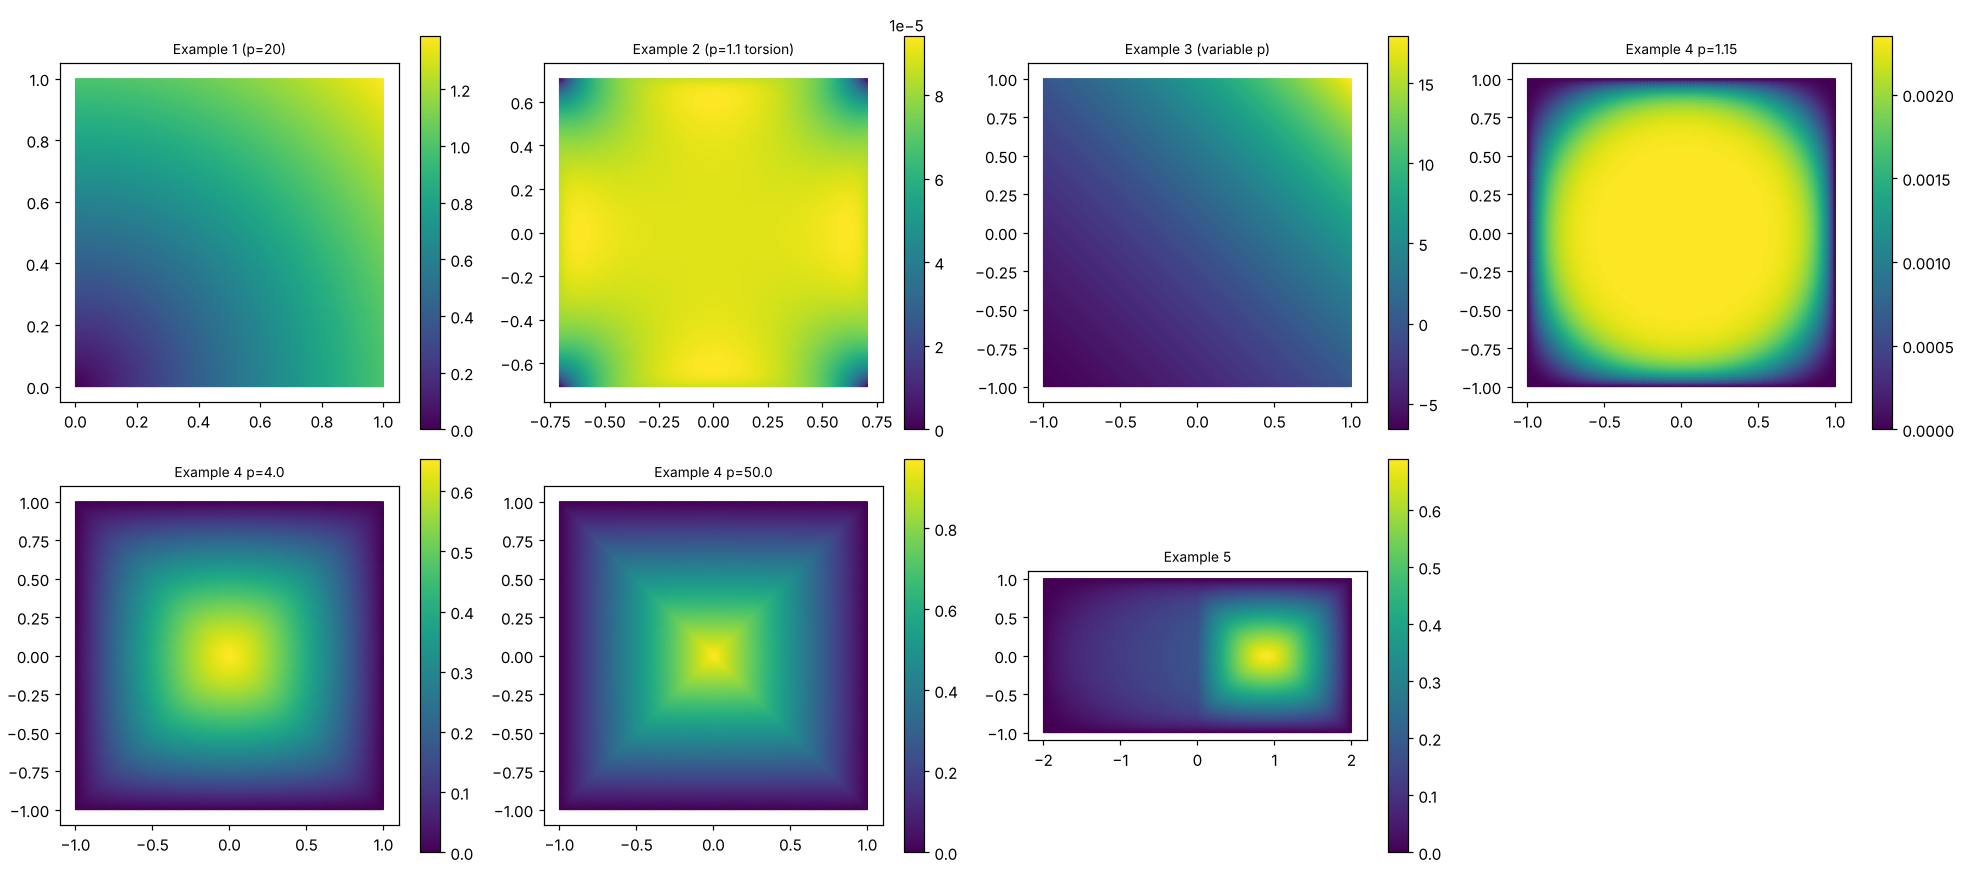
\includegraphics[width=\textwidth]{paper_examples.png}
\caption{Computed solutions of Examples 1--5. Top: Examples 1, 2, 3 and Example 4 with $p=1.15$. Bottom: Example 4 with $p=4$ and $p=50$, and Example 5.}\label{fig.examples}
\end{figure}

\begin{figure}[ht]
\centering
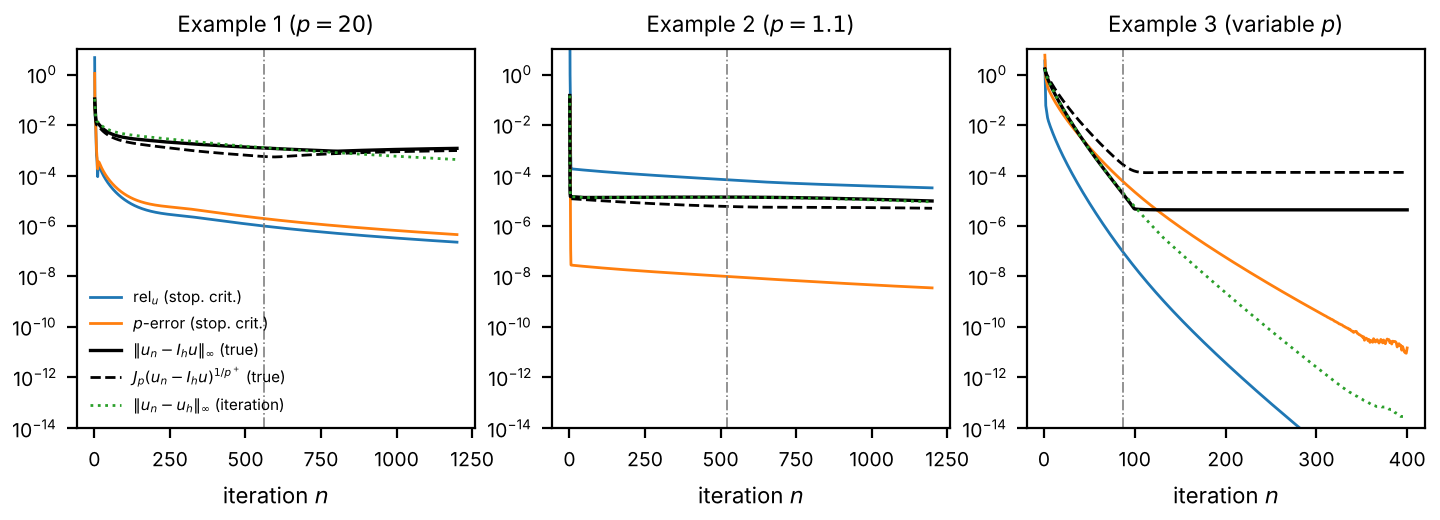
\includegraphics[width=\textwidth]{ex_errors.png}
\caption{Examples 1--3 ($100\times100$ cells). Stopping quantities \texttt{rel\_u} and \texttt{p\_error} (coloured), nodal error with respect to the exact solution (black; solid: maximum norm, dashed: $\mathcal M_{p_h}$), and distance to a reference iterate (green dotted: $4000$ iterations for Examples 1--2, $1500$ for Example 3; for Examples 1--2 the reference is itself not fully converged). The vertical line marks the iteration at which the stopping rule of Table~\ref{tab.examples} is met.}\label{fig.exerrors}
\end{figure}

Some comments are in order.
\begin{itemize}
\item In Examples 1 and 2 the error at the stopping iteration is dominated by the iteration error, not by the discretisation error. In Example~1 the iterate at the stop is still at distance $1.27\times10^{-3}$ (maximum norm) from the reference iterate, and the smaller error at the stop than after $4000$ iterations is the result of a cancellation between iteration and discretisation errors; after $4000$ iterations the primal residual $\|\nabla u_n-\nu_n\|$ is still $2.3\times10^{-3}$.
\item In Example~2 the solution is very small, $\max u=c_p\approx8.9\times10^{-5}$, so that only relative errors are meaningful. The absolute criterion \texttt{p\_error} $<10^{-8}$ stops the iteration when the relative maximum error is $15.7\%$, almost all of which is iteration error (the distance to the reference iterate is $1.38\times10^{-5}$); after $4000$ iterations the relative error is $1.3\%$ and the iteration is still not converged (\texttt{rel\_u} $\approx4\times10^{-6}$). The scale-invariant criterion \texttt{rel\_u} is more adequate here: it correctly signals that the iterate is still changing (\texttt{rel\_u} $<10^{-5}$ is not reached within $1200$ iterations), whereas \texttt{p\_error} $<10^{-6}$ is already met at the fourth iteration. The slow convergence for $p$ close to $1$ is analysed in Section~\ref{sec.pto1}.
\item In Example~3 the error at termination depends on the tolerance: with \texttt{rel\_u} $<10^{-5}$, $10^{-6}$, $10^{-7}$, $10^{-8}$ the maximum nodal error is $1.23\times10^{-3}$, $1.61\times10^{-4}$, $1.90\times10^{-5}$ and $4.47\times10^{-6}$, respectively, while the converged value is $4.36\times10^{-6}$. Under mesh refinement with tolerance $10^{-10}$ the error decreases as $h^2$ (Table~\ref{tab.varp}). The value of $\mathcal M_{p_h}(e)$, much larger than $\|e\|_\infty$, illustrates that $\mathcal M_{p_h}$ is not a norm (Section~\ref{sec.stopping}).
\item In Example~4 the solution is small and has a plateau-like profile with steep gradients near the boundary for $p$ close to $1$, and it approaches a pyramid-shaped profile as $p$ grows. In Example~5 the solution has a plateau-like profile in the region where $p=1.2$ and a pronounced maximum in the region where $p=4$.
\end{itemize}

\subsection{Torsion on the disk: order of convergence as a function of \texorpdfstring{$p$}{p}}\label{sec.torsion}
On the unit disk $B_1$ the problem $-\Delta_pu=1$, $u=0$ on $\partial B_1$, has the explicit solution
\begin{equation}\label{eq.torsion}
u(x)=c_p\big(1-|x|^{\frac p{p-1}}\big),\qquad c_p=\frac{p-1}p\,2^{-\frac1{p-1}},\qquad \nabla u=-\Big(\frac{|x|}2\Big)^{\frac1{p-1}}\frac{x}{|x|}.
\end{equation}
We computed it on sequences of unstructured meshes of the disk produced by \texttt{disk\_mesh} with $h=0.1,0.05,0.025,0.0125$ (362 to 23\,227 nodes) for $p\in\{1.3,1.5,2,3,4,6\}$, and with $h=0.2,0.1,0.05,0.025$ (88 to 5809 nodes) for $p\in\{1.1,1.2\}$. Boundary values $g=u$ are imposed at the boundary nodes. The stopping rule is \texttt{rel\_u} $<10^{-10}$; for $p\in\{1.1,1.2\}$ the iteration was limited to $6000$ iterations. Table~\ref{tab.order} gives the true relative errors and the observed orders, together with the number of iterations, and Figure~\ref{fig.order} shows them graphically.

\begin{table}[ht]
\centering
\caption{Torsion problem on the unit disk: true relative errors $\|u-u_h\|_{L^2}$ and $\|\nabla(u-u_h)\|_{L^p}$ on the finest mesh of each sequence, observed orders $t$ (least-squares fit over the three finest meshes) and number of iterations on the four meshes (coarsest to finest). $^*$: the tolerance $10^{-10}$ was not reached within $6000$ iterations.}\label{tab.order}
\small
\setlength{\tabcolsep}{3.5pt}
\begin{tabular}{lcccccccc}
\toprule
$p$ & 1.1 & 1.2 & 1.3 & 1.5 & 2 & 3 & 4 & 6\\
finest $h$ & 0.025 & 0.025 & 0.0125 & 0.0125 & 0.0125 & 0.0125 & 0.0125 & 0.0125\\
\midrule
$L^2$ error & 5.96e-3 & 1.60e-3 & 2.11e-4 & 1.15e-4 & 7.04e-5 & 5.95e-5 & 6.13e-5 & 7.13e-5\\
$t$ ($L^2$) & 1.84 & 1.98 & 2.00 & 2.01 & 2.00 & 2.00 & 2.00 & 2.00\\
gradient error & 6.02e-2 & 3.15e-2 & 1.09e-2 & 7.30e-3 & 5.14e-3 & 6.10e-3 & 1.41e-2 & 6.36e-2\\
$t$ (gradient) & 1.01 & 1.02 & 1.02 & 1.02 & 1.02 & 1.00 & 0.82 & 0.46\\
\midrule
iterations & 6000$^*$ & 6000$^*$ & 3237 & 207 & 2 & 64 & 85 & 94\\
 & 6000$^*$ & 6000$^*$ & 1460 & 194 & 2 & 80 & 130 & 172\\
 & 6000$^*$ & 6000$^*$ & 845 & 151 & 2 & 87 & 146 & 204\\
 & 6000$^*$ & 3863 & 480 & 75 & 2 & 109 & 219 & 343\\
\bottomrule
\end{tabular}
\end{table}

\begin{figure}[ht]
\centering
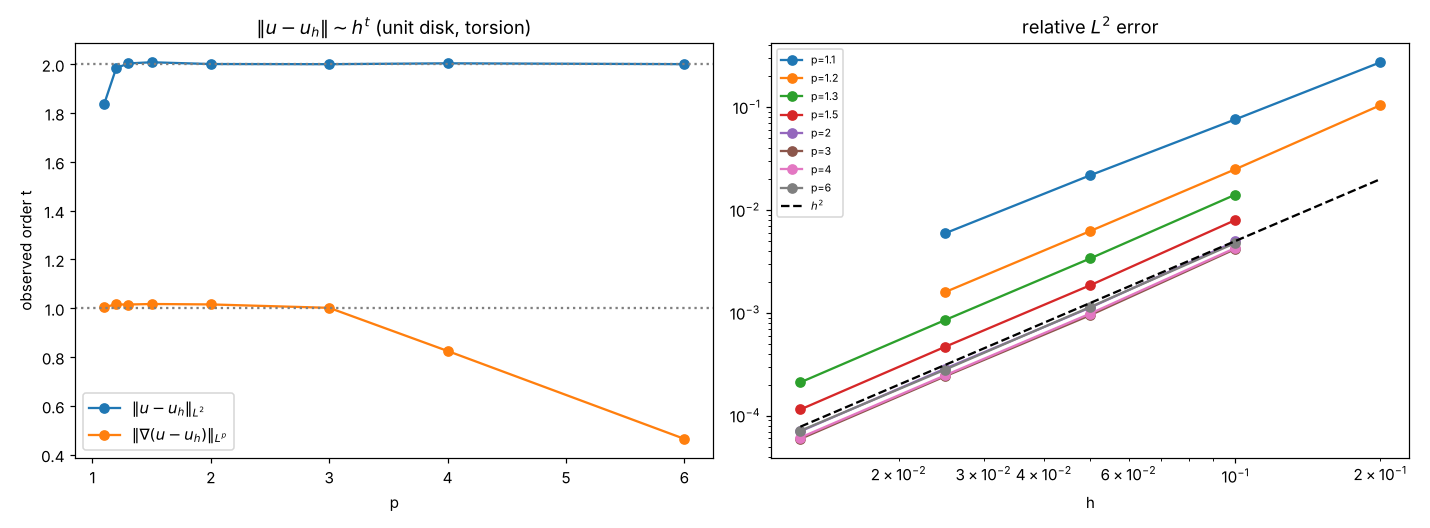
\includegraphics[width=\textwidth]{convergence_order_true.png}
\caption{Torsion problem on the unit disk, true errors. Left: observed orders $t(p)$ of the relative errors $\|u-u_h\|_{L^2}$ and $\|\nabla(u-u_h)\|_{L^p}$ (Table~\ref{tab.order}). Right: relative $L^2$ error against $h$ for each $p$; the dashed line has slope $2$.}\label{fig.order}
\end{figure}

The observed order of the $L^2$ error is $2.00\pm0.01$ for $p$ between $1.3$ and $6$, $1.98$ for $p=1.2$ and $1.84$ for $p=1.1$; for $p=1.1$ the meshes are coarse relative to the boundary layer discussed below and the iteration did not reach the tolerance. The gradient error has order close to $1$ for $p\le3$, and smaller orders for $p=4$ ($0.82$) and $p=6$ ($0.46$, with fluctuating pair orders). The latter is consistent with the limited smoothness of $u$ at the origin, where $|\nabla u|\sim|x|^{1/(p-1)}$: a scaling argument for the interpolation error on the triangles near the origin gives the exponent $\min\{1,\frac1{p-1}+\frac2p\}$, that is, $1$ for $p\le3$, $0.83$ for $p=4$ and $0.53$ for $p=6$. We have not analysed this further. We note that nodal error measures such as $\|I_hu-u_h\|_{L^2}$ can be misleading here: on these nearly equilateral meshes they show supercloseness (for instance a nodal $L^2$ order of about $2.5$ for $p=2$, where the true order is $2.00$).

As $p\to1$ the \emph{constant} deteriorates: the relative $L^2$ error at $h=0.05$ is $9.9\times10^{-4}$ for $p=4$, $1.13\times10^{-3}$ for $p=2$, $1.86\times10^{-3}$ for $p=1.5$, $3.39\times10^{-3}$ for $p=1.3$, $6.26\times10^{-3}$ for $p=1.2$ and $2.18\times10^{-2}$ for $p=1.1$. A heuristic explanation is visible in \eqref{eq.torsion}: $u/c_p=1-|x|^{p/(p-1)}$ is almost constant except in a layer near $\partial B_1$ of width of order $p-1$, where its second radial derivative is of order $p/(p-1)^2$. The asymptotic regime can only be expected when $h$ is small compared with $p-1$.

For $p=1.1$ (all meshes) and $p=1.2$ ($h=0.2,0.1,0.05$) the tolerance was not reached within $6000$ iterations, so the corresponding errors contain an iteration component (see Section~\ref{sec.pto1}). The number of iterations is not independent of the mesh (Table~\ref{tab.order}): it grows under refinement for $p\ge3$ (from $85$ to $219$ for $p=4$) and decreases for $p=1.3$ and $p=1.5$. For $p=2$ the iteration stops after two iterations for the reason explained in Section~\ref{sec.pto1}.

Figure~\ref{fig.disk} shows, for $p=4$, the computed and exact solutions and the error, which is largest near the centre of the disk, where $\nabla u$ vanishes and the equation degenerates.

\begin{figure}[ht]
\centering
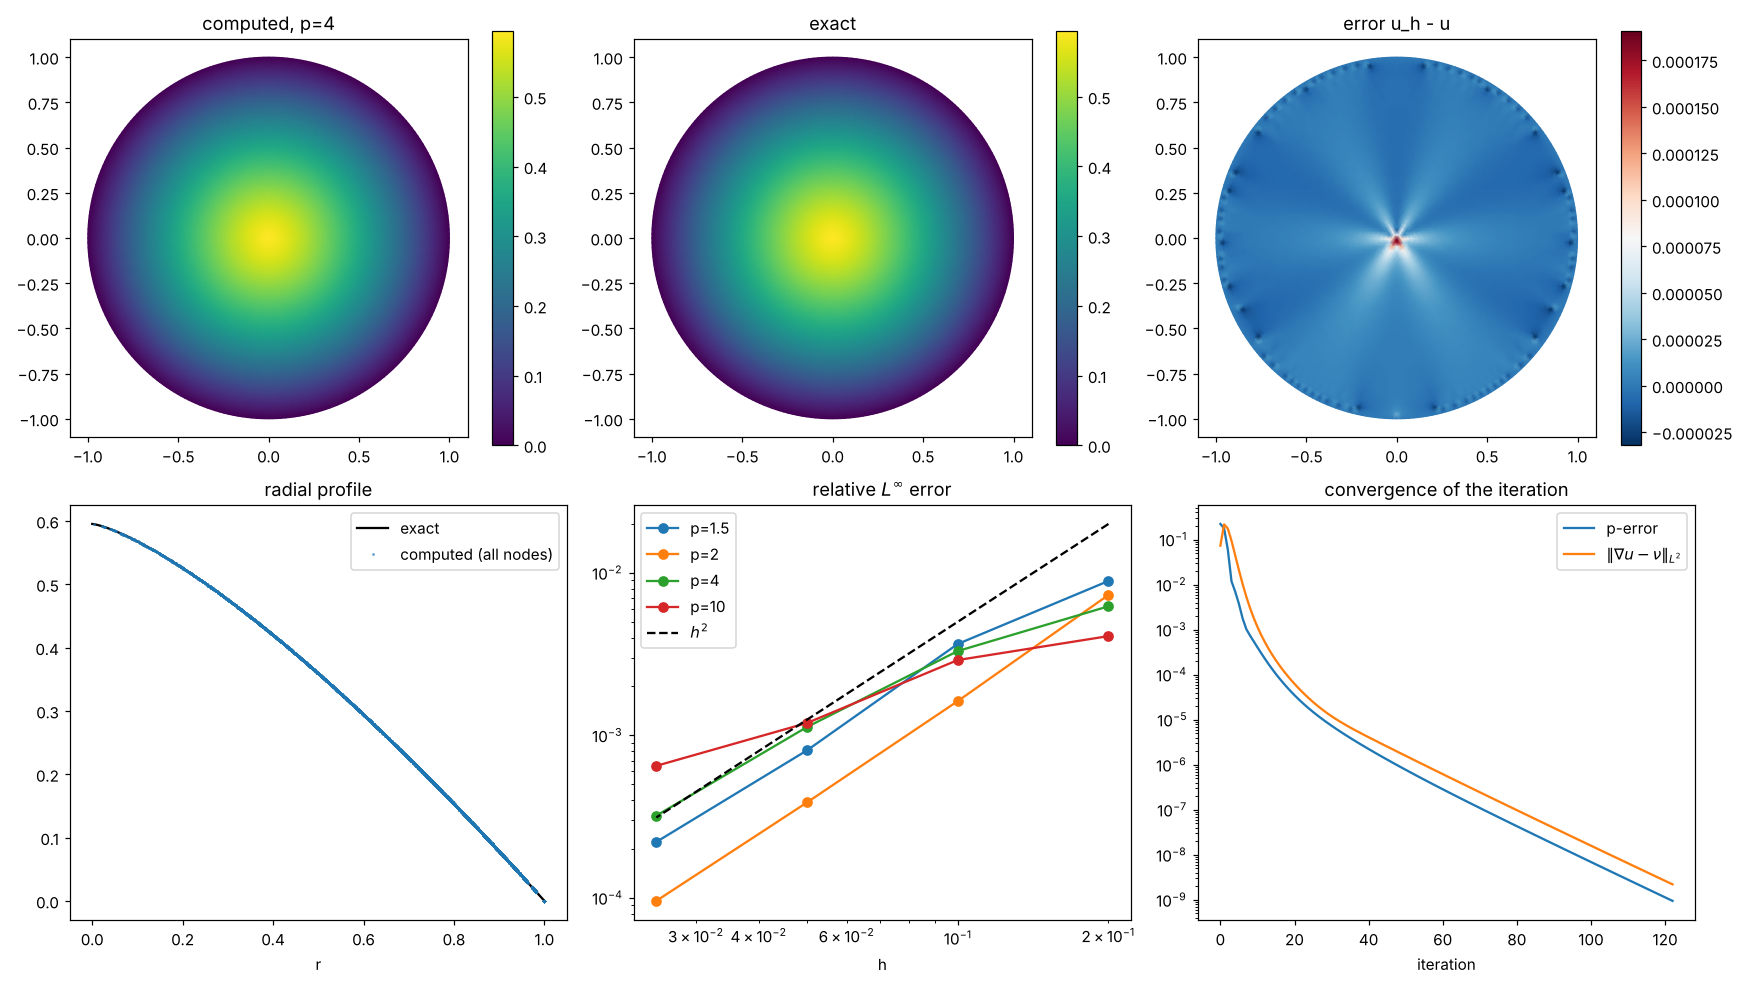
\includegraphics[width=\textwidth]{torsion_disk.png}
\caption{Torsion problem on the unit disk. Top: computed solution for $p=4$, exact solution, and error $u_h-u$ at the nodes. Bottom: radial profile (all nodes), relative nodal maximum error against $h$ for several values of $p$, and stopping quantities along the iteration.}\label{fig.disk}
\end{figure}

\subsection{Behaviour of the iteration as \texorpdfstring{$p\to1$}{p -> 1}}\label{sec.pto1}
We now study the number of iterations. We consider $-\Delta_pu=2$ on the unit disk, with exact solution $u(x)=\frac{p-1}p\big(1-|x|^{p/(p-1)}\big)$ (so that $\max u$ does not tend to zero as $p\to1$), a fixed mesh with $h=0.05$ (1452 nodes), and $r=1$. We monitor the relative primal residual $\|\nabla u_n-\nu_n\|_{L^2}/\|\nabla u_n\|_{L^2}$ and define its linear contraction factor $\rho(p)$ as $\exp$ of the slope of a least-squares fit of $\log(\text{residual})$ against $n$ on the window where the residual lies between $10^{-6}$ and $10^{-3}$. The results are in Table~\ref{tab.rho} and Figure~\ref{fig.pto1}. For $p$ close to $1$ the estimate of $\rho$ depends on the fitting window and on the length of the run in the fourth decimal (for $p=1.1$ we obtained values between $0.9989$ and $0.9995$).

\begin{table}[ht]
\centering
\caption{Iteration on the unit disk, $h=0.05$, $r=1$: contraction factor $\rho(p)$ of the primal residual and number of iterations needed to reach \texttt{rel\_u} $<10^{-8}$. For $p=2$ see the text.}\label{tab.rho}
\small
\setlength{\tabcolsep}{3.2pt}
\begin{tabular}{lccccccccccccc}
\toprule
$p$ & 6 & 4 & 3 & 2.5 & 2 & 1.8 & 1.6 & 1.5 & 1.4 & 1.3 & 1.2 & 1.1 & 1.05 \\
\midrule
$\rho(p)$ & .834 & .789 & .670 & .530 & .5 & .547 & .724 & .923 & .979 & .994 & .998 & .999 & .9995\\
iterations & 69 & 57 & 39 & 26 & 2 & 28 & 35 & 40 & 48 & 89 & 200 & 680 & 2113\\
\bottomrule
\end{tabular}

\smallskip
{\footnotesize Further iteration counts: $p=1.15$: 339; $p=1.07$: 1226; $p=1.03$: 4824; $p=1.02$ and $p=1.01$: not reached within $8000$ iterations.}
\end{table}

\begin{figure}[ht]
\centering
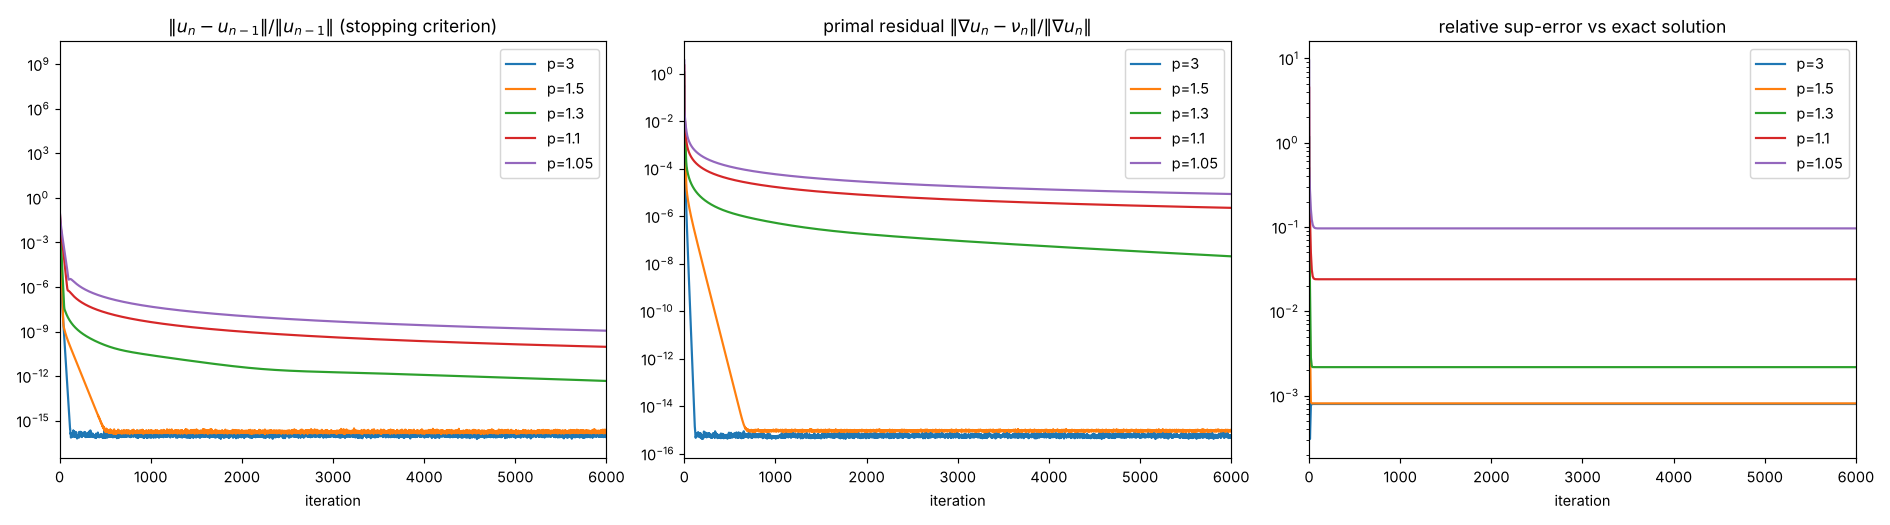
\includegraphics[width=\textwidth]{p_to_1_iteration.png}
\caption{$-\Delta_pu=2$ on the unit disk, $h=0.05$, $r=1$, $6000$ iterations without stopping. Left: \texttt{rel\_u}; centre: relative primal residual; right: relative maximum error with respect to the exact solution.}\label{fig.pto1}
\end{figure}

For $p=2$ and $r=1$ the behaviour can be computed by hand. By Proposition~\ref{prop.derivation}(c), $\eta^{n+1}=\nu^n$, so the right-hand side of \eqref{eq.disc.u} reduces to $F_i$ for $n\ge2$; with $\nu^0=\eta^1=0$ this holds also for $n=1$. Hence $u^n$ is the discrete solution for every $n\ge1$ and \texttt{rel\_u} vanishes at the second iteration, while $\nu^n=(\nu^{n-1}+\nabla u^n)/2$, so that $\nabla u^n-\nu^n$ is exactly halved at each iteration ($\rho(2)=1/2$). Away from $p=2$ the contraction factor varies mildly for $p>2$ ($0.53$ at $p=2.5$, $0.83$ at $p=6$) and increases sharply as $p\to1$, where it approaches $1$ and the number of iterations grows quickly. Two further observations are relevant for practice.

\begin{itemize}
\item The approximation $u_n$ stabilises much earlier than the auxiliary variables: the criterion \texttt{rel\_u} $<10^{-8}$ is reached after 89 iterations for $p=1.3$ although $\rho(1.3)=0.994$, and at that point the relative primal residual is still of order $2$--$3\times10^{-5}$ for $p\le1.3$; it continues to decrease slowly afterwards (Figure~\ref{fig.pto1}, centre). Thus a converged flag based on \texttt{rel\_u} certifies only that the increments of $u_n$ are small, and the absence of the flag (as in Section~\ref{sec.torsion} for $p\le1.2$) does not by itself mean that $u_n$ is inaccurate.
\item At fixed $h$, the error with respect to the exact solution grows as $p\to1$: the relative maximum error is $8\times10^{-4}$ for $p=1.5$, $2.4\times10^{-2}$ for $p=1.1$ and $9.6\times10^{-2}$ for $p=1.05$ (Figure~\ref{fig.pto1}, right). In these long runs the error no longer changes after the first few hundred iterations, so it is a discretisation error, consistent with the unresolved boundary layer described in Section~\ref{sec.torsion}; it decreases under mesh refinement.
\end{itemize}

The augmented Lagrangian parameter $r$ affects the speed but not the qualitative behaviour (Table~\ref{tab.r}, a single problem on a single mesh): for $p=1.1$, $r\approx3$ roughly halves the number of iterations with respect to $r=1$, while both smaller and larger values of $r$ increase it.

\begin{table}[ht]
\centering
\caption{Iterations needed to reach \texttt{rel\_u} $<10^{-8}$ for $p=1.1$ on the unit disk ($h=0.05$) as a function of $r$.}\label{tab.r}
\begin{tabular}{lcccccc}
\toprule
$r$ & 0.1 & 0.3 & 1 & 3 & 10 & 30\\
\midrule
iterations & 2322 & 1292 & 680 & 364 & 987 & 2698\\
\bottomrule
\end{tabular}
\end{table}

\subsection{Variable exponents with explicit solutions}\label{sec.varp}
We consider four problems with nonconstant $p$ and known solution, computed with \texttt{rel\_u} $<10^{-10}$ (the tolerance was reached in all cases):
\begin{enumerate}
\item[(V1)] \emph{Smooth manufactured solution} on the unit disk: $p(x,y)=2+0.8x$ (so that $p$ takes values on both sides of $2$), $u=e^{x/2}(1+y/2)$, $f=-\dvg(|\nabla u|^{p-2}\nabla u)$ computed symbolically, load vector with the edge-midpoint rule.
\item[(V2)] \emph{Radial torsion} on the unit disk with $p(x)=1.5+1.5|x|$. For a radial exponent $p(\rho)$, $\rho=|x|$, integrating the equation $-\rho^{-1}(\rho|u'|^{p-2}u')'=1$ gives $|u'|^{p-2}u'=-\rho/2$, hence $u'(\rho)=-(\rho/2)^{1/(p(\rho)-1)}$ and $u(\rho)=\int_\rho^1(s/2)^{1/(p(s)-1)}\,ds$, which we evaluate by numerical quadrature on a fine grid.
\item[(V3)] \emph{Example 3} of Section~\ref{sec.examples} on $(-1,1)^2$, with $n\times n$ cells, $n=10,20,40,80,160$ ($h=2/n$).
\item[(V4)] \emph{Radial torsion with a discontinuous exponent}: $p=1.5$ for $|x|<0.5$ and $p=3$ for $|x|\ge0.5$. The formula of (V2) remains valid, since only the continuity of the flux $|u'|^{p-2}u'=-\rho/2$ is used. The solution has a kink at $|x|=0.5$ ($u'(0.5^-)=-0.0625$, $u'(0.5^+)=-0.5$), and the interface is not aligned with the mesh.
\end{enumerate}
The disk meshes are those of Section~\ref{sec.torsion} with $h=0.2,\dots,0.0125$. The relative true $L^2$ errors and the relative nodal maximum errors are reported in Table~\ref{tab.varp} and Figure~\ref{fig.varp}.

\begin{table}[ht]
\centering
\caption{Variable exponents: relative true $L^2$ errors and relative nodal maximum errors, and observed orders over the three finest meshes. For (V3), $h=2/n$.}\label{tab.varp}
\small
\setlength{\tabcolsep}{4pt}
\begin{tabular}{lcccccccc}
\toprule
& \multicolumn{2}{c}{(V1) smooth} & \multicolumn{2}{c}{(V2) $p=1.5+1.5|x|$} & \multicolumn{2}{c}{(V3) Example 3} & \multicolumn{2}{c}{(V4) jump}\\
\cmidrule(lr){2-3}\cmidrule(lr){4-5}\cmidrule(lr){6-7}\cmidrule(lr){8-9}
$h$ & $L^2$ & max & $L^2$ & max & $L^2$ & max & $L^2$ & max\\
\midrule
0.2    & 1.04e-3 & 4.25e-4 & 2.02e-2 & 8.66e-3 & 2.32e-3 & 2.40e-5 & 5.15e-2 & 5.56e-2\\
0.1    & 2.24e-4 & 1.08e-4 & 4.83e-3 & 1.76e-3 & 5.78e-4 & 6.05e-6 & 9.17e-3 & 2.56e-2\\
0.05   & 5.22e-5 & 2.00e-5 & 1.10e-3 & 3.90e-4 & 1.45e-4 & 1.52e-6 & 6.26e-3 & 1.37e-2\\
0.025  & 1.25e-5 & 5.05e-6 & 2.81e-4 & 9.52e-5 & 3.61e-5 & 3.79e-7 & 1.65e-3 & 7.80e-3\\
0.0125 & 3.10e-6 & 1.83e-6 & 6.86e-5 & 2.33e-5 & 9.03e-6 & 9.49e-8 & 7.90e-4 & 3.94e-3\\
\midrule
order $t$ & 2.04 & 1.72 & 2.00 & 2.03 & 2.00 & 2.00 & 1.49 & 0.90\\
\bottomrule
\end{tabular}
\end{table}

\begin{figure}[ht]
\centering
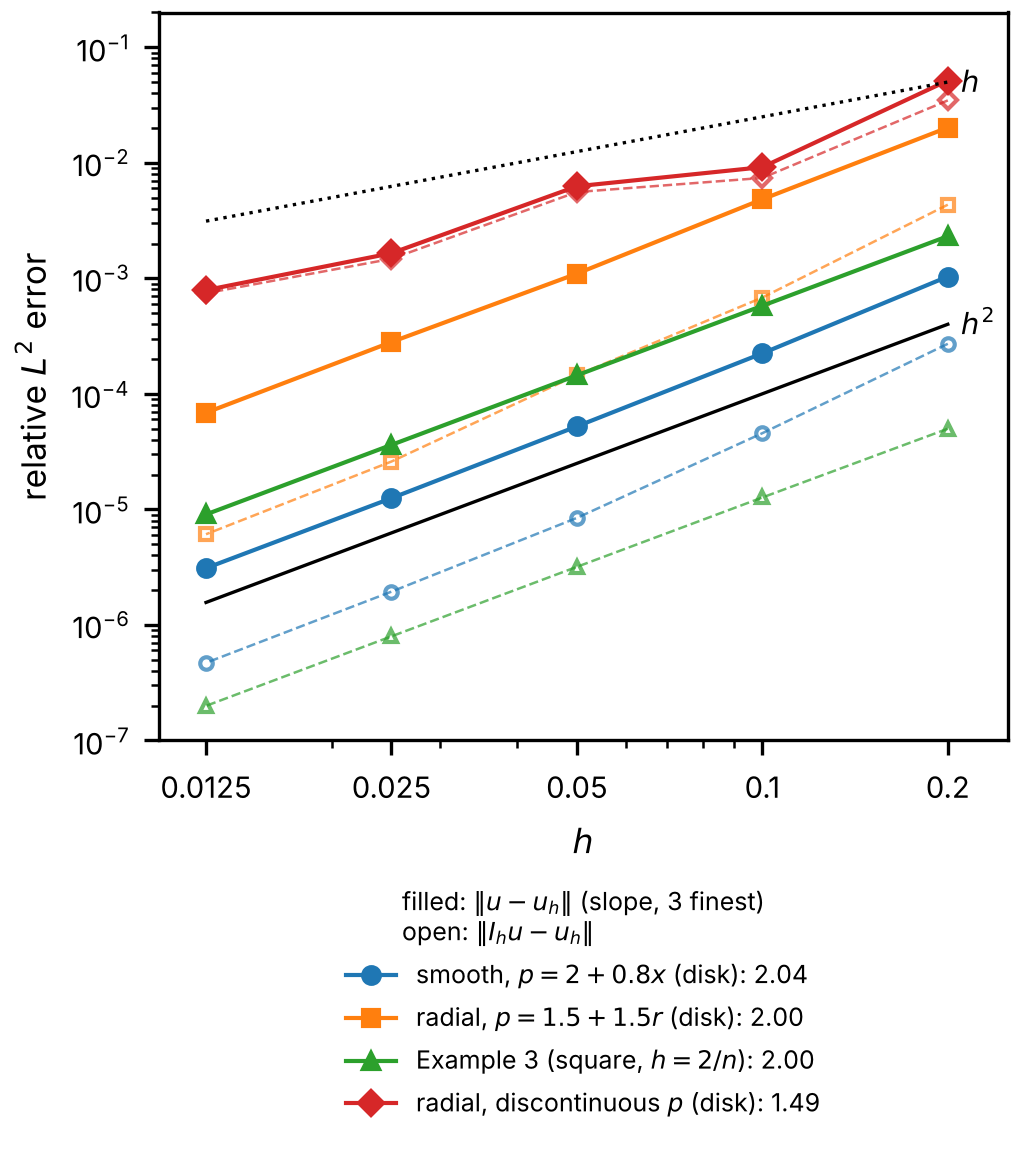
\includegraphics[width=0.62\textwidth]{variable_p_order.png}
\caption{Relative $L^2$ error against $h$ for the variable exponents (V1)--(V4). Filled markers: true error $\|u-u_h\|_{L^2(\Omega_h)}$; open markers: nodal error $\|I_hu-u_h\|_{L^2}$. Slopes in the legend are least-squares fits over the three finest meshes. Reference slopes $h^2$ and $h$.}\label{fig.varp}
\end{figure}

For the continuous exponents (V1)--(V3) the observed order of the true $L^2$ error is $2$ (pair orders between $1.97$ and $2.21$). In (V1) the order of the nodal maximum error is irregular on the finest meshes (pair orders $1.98$ and $1.46$), which we attribute to the irregularity of the meshes; we do not draw conclusions from the fitted value $1.72$. For (V3), the nodal $L^2$ errors $\|I_hu-u_h\|_{L^2}$ (Figure~\ref{fig.varp}, open triangles) are about $45$ times smaller than the true ones, an example of the supercloseness mentioned in Section~\ref{sec.measures}.

For the discontinuous exponent (V4) the maximum error has order close to $1$ (pair orders $1.12$, $0.90$, $0.81$, $0.98$), while the $L^2$ pair orders are erratic ($2.49$, $0.55$, $1.92$, $1.06$, fit $1.49$). This is what one expects from piecewise linear approximation of a function with a kink across a curve that is not aligned with the mesh: the best approximation error is of order $h$ in $L^\infty$ and of order $h^{3/2}$ in $L^2$, since the error is of order $h$ on a band of area of order $h$. In addition, sampling $p$ at the barycentres assigns the wrong exponent to some of the triangles crossed by the interface. As a diagnostic (script \texttt{examples/p\_sampling\_diagnostic.py} of the repository) we replaced the barycentre value $p_T=p(x_T)$ by the arithmetic or the harmonic mean of $p$ over an $8\times8$ barycentric sub-grid of each triangle (Table~\ref{tab.avg}). The arithmetic mean reduces the true $L^2$ error by a factor between $1.2$ and $2.3$ and the nodal maximum error by a factor of about $4$ ($1.4$ and $4.5$ at $h=0.0125$); the harmonic mean gives smaller improvements. The observed orders, however, stay between $1$ and $1.5$ (arithmetic mean: $1.11$ in $L^2$ and $0.96$ for the maximum error): the limiting factor is the unresolved interface, where $u$ has a kink, and not only the sampling of $p$. For exponents that jump across curves, interface-fitted meshes should therefore be used when higher accuracy is needed.

\begin{table}[ht]
\centering
\caption{Problem (V4): relative true $L^2$ error / relative nodal maximum error for three ways of defining $p_T$: value at the barycentre, arithmetic mean and harmonic mean over an $8\times8$ sub-grid of $T$. Last row: observed orders over the three finest meshes.}\label{tab.avg}
\small
\begin{tabular}{lccc}
\toprule
$h$ & barycentre & arithmetic mean & harmonic mean\\
\midrule
0.1    & 9.17e-3 / 2.56e-2 & 7.51e-3 / 6.41e-3 & 1.11e-2 / 1.23e-2\\
0.05   & 6.26e-3 / 1.37e-2 & 2.69e-3 / 3.35e-3 & 4.11e-3 / 6.31e-3\\
0.025  & 1.65e-3 / 7.80e-3 & 1.10e-3 / 1.58e-3 & 1.61e-3 / 3.17e-3\\
0.0125 & 7.90e-4 / 3.94e-3 & 5.74e-4 / 8.80e-4 & 7.41e-4 / 1.64e-3\\
\midrule
order $t$ & 1.49 / 0.90 & 1.11 / 0.96 & 1.24 / 0.97\\
\bottomrule
\end{tabular}
\end{table}

\subsection{General domains}\label{sec.domains}
Since the implementation only needs the three mesh arrays, non-rectangular domains require no change in the solver. Figure~\ref{fig.domains} shows three examples of the torsion problem $-\Delta_{p(x)}u=1$, $u=0$ on $\partial\Omega$: an L-shaped domain meshed with \texttt{polygon\_mesh} ($p=3$), an annulus $\{0.5<|x|<2\}$ treated as a polygon with a polygonal hole ($p(x)=1.5+0.5|x|$), and the union of two overlapping discs described by a signed distance function and meshed with \texttt{sdf\_mesh} ($p=1.3$ for $x<0$ and $p=4$ for $x\ge0$). These examples are qualitative: no exact solution is available. The computed solutions show the expected features: symmetry with respect to the diagonal in the L-shaped domain, radial symmetry in the annulus, and the flat profile in the region where $p$ is close to $1$ next to the peaked profile where $p=4$. Curved boundaries are approximated by polygons, which introduces a geometric error of order $h^2$ in the position of the boundary.

\begin{figure}[ht]
\centering
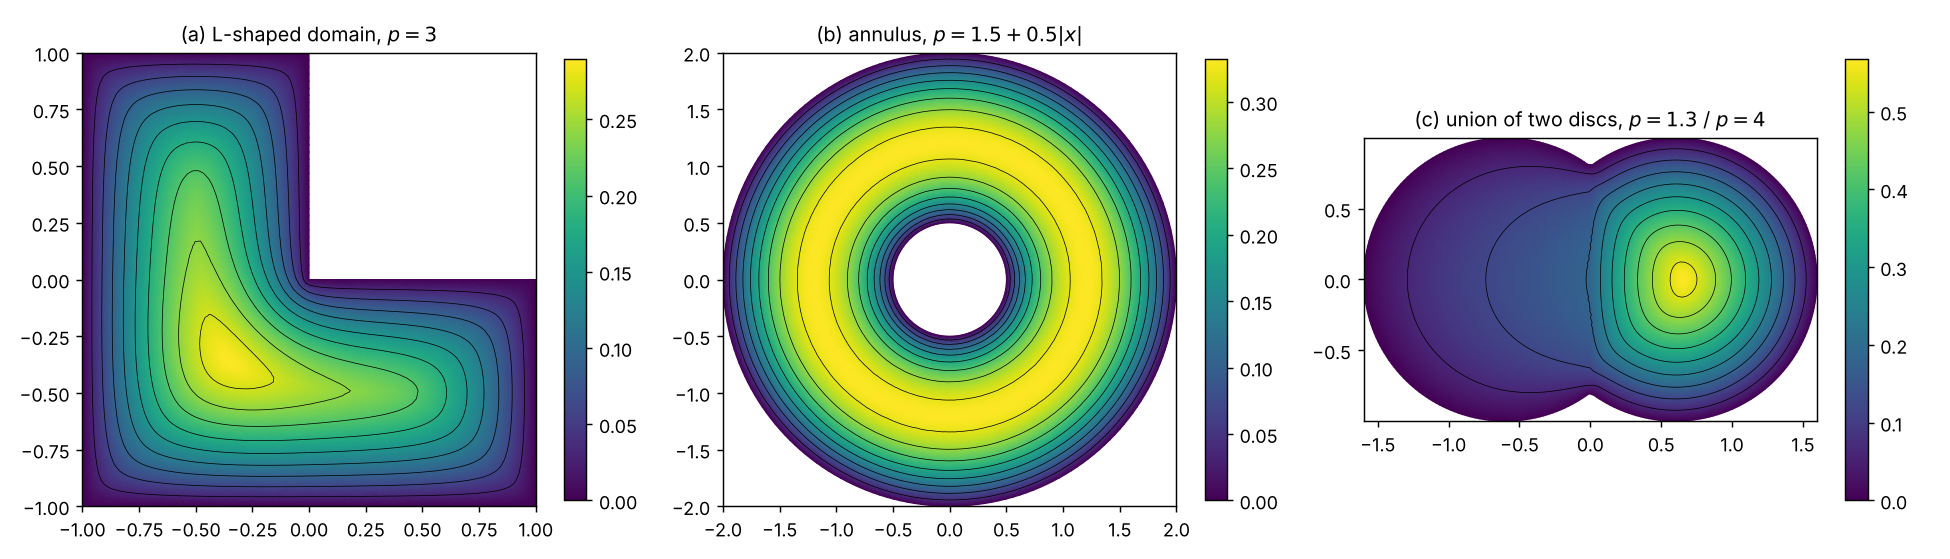
\includegraphics[width=\textwidth]{general_domains.png}
\caption{Torsion problems on non-rectangular domains (\texttt{rel\_u} $<10^{-8}$; about 6000--6900 nodes): (a) L-shaped domain, $p=3$; (b) annulus, $p(x)=1.5+0.5|x|$; (c) union of two discs, $p=1.3$ for $x<0$ and $p=4$ for $x\ge0$. Level lines are drawn in black.}\label{fig.domains}
\end{figure}

\subsection{On the stopping criteria}\label{sec.stopping.discussion}
Both criteria of Section~\ref{sec.stopping} measure increments of $u_n$, not errors, and the experiments above show their limitations.
\begin{itemize}
\item \emph{No fixed relation with the error.} The ratio between the error and the stopping quantity is not constant along the iteration: the stopping quantities tend to zero, whereas the error tends to the discretisation error (Figure~\ref{fig.exerrors}). At the stopping iteration the ratio $\mathcal M_{p_h}(u_n-I_hu)/\mathcal M_{p_h}(u_n-u_{n-1})$ was about $287$, $594$ and $4.7$ in Examples 1, 2 and 3, respectively. A roughly constant ratio can only be observed during a transient phase in which the iteration error dominates.
\item \emph{Tolerance dependence.} The error at termination can be dominated by the tolerance (Example~3: $1.23\times10^{-3}$ with $10^{-5}$ and $4.47\times10^{-6}$ with $10^{-8}$), so the tolerance has to be chosen in relation to the expected discretisation error. In the convergence studies we used $10^{-10}$.
\item \emph{Scaling.} \texttt{rel\_u} is invariant under scaling of the solution, whereas \texttt{p\_error} is absolute and, for variable $p$, not homogeneous. For solutions of very small size (Example~2) the absolute criterion is satisfied far too early; for solutions of large size it may be very demanding.
\item \emph{Slow convergence.} When the contraction factor is close to $1$ (Section~\ref{sec.pto1}), small increments do not imply a small distance to the limit: for a sequence converging linearly with factor $\rho$, the distance to the limit can be up to $\rho/(1-\rho)$ times the last increment, which is of order $10^3$ for $p=1.1$. On the other hand, in our experiments $u_n$ often stabilises long before the primal residual $\|\nabla u_n-\nu_n\|$ becomes small.
\end{itemize}
It is therefore advisable to monitor also the primal residual and the energy, which are recorded by the solver, to prefer the scale-invariant criterion \texttt{rel\_u} to the absolute one, and to check, when possible, that a reduction of the tolerance does not change the result. Relative primal and dual residuals, as customary for the alternating direction method of multipliers \cite{Boyd}, are a natural alternative that we have not tested.

%=====================================================================
\section{Conclusions}\label{sec.conclusions}
%=====================================================================

We have presented the decomposition--coordination method for the $p(x)$-Laplacian with a general augmented Lagrangian parameter $r$, derived it from the optimality conditions of the augmented Lagrangian, and recalled the convergence result available when $p(x)\ge2$, under a regularity assumption on the solution that guarantees the existence of a saddle point. Each iteration requires one solution of a linear system with a fixed, prefactorised matrix and the solution of decoupled scalar equations with explicitly bracketed roots. The vectorised Python implementation \texttt{pxlaplace} works on arbitrary triangulations of planar domains.

The experiments indicate the following. For the torsion problem on the disk, the $L^2$ error of the piecewise linear approximation has observed order $2$ for $p$ between $1.2$ and $6$ ($1.84$ for $p=1.1$, where the meshes are coarse relative to the boundary layer and the iteration did not reach its tolerance), and the gradient error has order close to $1$ for $p\le3$ and smaller orders for $p=4,6$, consistent with the limited smoothness of the solution at the origin. As $p\to1$ the error constant deteriorates, which we attribute to a boundary layer of width of order $p-1$. The iteration converges numerically also for $1<p<2$, but its contraction factor tends to $1$ as $p\to1$; it can be improved moderately by the choice of $r$, and the number of iterations depends on the mesh. For continuous variable exponents the observed $L^2$ order is $2$, as for constant exponents, whereas for an exponent that jumps across a curve not aligned with the mesh the accuracy is limited to first order in the maximum norm. Non-rectangular domains require no modification of the solver. Finally, the error at termination can be dominated by the iteration error when the stopping tolerance is not chosen in relation to the discretisation error, in particular for $p$ close to $1$ and for very large $p$.

The study has several limitations. Convergence of the iteration for $1<p<2$ is not proved (Open question~\ref{q.p<2}). The observed orders are obtained from fits over three meshes of unstructured, non-nested sequences, and they fluctuate from pair to pair. The contraction factors were measured on a single mesh and a single problem. The results depend on the stopping tolerance, and the stopping criteria measure increments, not errors. Curved domains are approximated by polygons, and errors are measured on the polygonal domain. For $p$ close to $1$ both the number of iterations and the mesh resolution needed to resolve boundary layers grow quickly; preconditioning or acceleration of the iteration, residual-based stopping criteria, adaptive mesh refinement and interface-fitted meshes for discontinuous exponents are natural directions for further work.

\section*{Acknowledgements}
The authors thank I.~Ojea for useful discussions and for help with an early version of the code. This research was partially supported by CONICET PIP N\textsuperscript{o} 11220150100032CO and by ANPCyT, PICT 2016-1022.

%=====================================================================
\begin{thebibliography}{99}

\bibitem{BL} {\sc J. W. Barrett and W. B. Liu}, \emph{Finite element approximation of the $p$-Laplacian}, Math. Comp. 61 (1993), no. 204, 523--537.

\bibitem{D} {\sc L. C. Berselli, D. Breit and L. Diening}, \emph{Convergence analysis for a finite element approximation of a steady model for electrorheological fluids}, Numer. Math. 132 (2016), no. 4, 657--689.

\bibitem{Boyd} {\sc S. Boyd, N. Parikh, E. Chu, B. Peleato and J. Eckstein}, \emph{Distributed optimization and statistical learning via the alternating direction method of multipliers}, Found. Trends Mach. Learn. 3 (2011), no. 1, 1--122.

\bibitem{CZ} {\sc M. Caliari and S. Zuccher}, \emph{Quasi-Newton minimization for the $p(x)$-Laplacian problem}, J. Comput. Appl. Math. 309 (2017), 122--131.

\bibitem{CLR} {\sc Y. Chen, S. Levine and M. Rao}, \emph{Variable exponent, linear growth functionals in image restoration}, SIAM J. Appl. Math. 66 (2006), no. 4, 1383--1406.

\bibitem{DPLM} {\sc L. M. Del Pezzo, A. L. Lombardi and S. Mart\'{\i}nez}, \emph{Interior penalty discontinuous Galerkin FEM for the $p(x)$-Laplacian}, SIAM J. Numer. Anal. 50 (2012), no. 5, 2497--2521.

\bibitem{DPM} {\sc L. M. Del Pezzo and S. Mart\'{\i}nez}, \emph{The decomposition-coordination method for the $p(x)$-Laplacian}, preprint, arXiv:1401.2442 (2014).

\bibitem{DPM2} {\sc L. M. Del Pezzo and S. Mart\'{\i}nez}, \emph{Order of convergence of the finite element method for the $p(x)$-Laplacian}, IMA J. Numer. Anal. 35 (2015), no. 4, 1864--1887.

\bibitem{DHHR} {\sc L. Diening, P. Harjulehto, P. H\"ast\"o and M. R\r{u}\v{z}i\v{c}ka}, \emph{Lebesgue and Sobolev Spaces with Variable Exponents}, Lecture Notes in Mathematics 2017, Springer, Heidelberg, 2011.

\bibitem{FG} {\sc M. Fortin and R. Glowinski}, \emph{Augmented Lagrangian Methods: Applications to the Numerical Solution of Boundary-Value Problems}, Studies in Mathematics and its Applications 15, North-Holland, Amsterdam, 1983.

\bibitem{GaM} {\sc D. Gabay and B. Mercier}, \emph{A dual algorithm for the solution of nonlinear variational problems via finite element approximation}, Comput. Math. Appl. 2 (1976), no. 1, 17--40.

\bibitem{Glowinski} {\sc R. Glowinski}, \emph{Numerical Methods for Nonlinear Variational Problems}, 2nd printing, Scientific Computation, Springer, Berlin, 2008.

\bibitem{GM} {\sc R. Glowinski and A. Marrocco}, \emph{Sur l'approximation, par \'el\'ements finis d'ordre un, et la r\'esolution, par p\'enalisation-dualit\'e, d'une classe de probl\`emes de Dirichlet non lin\'eaires}, Rev. Fran\c{c}aise Automat. Informat. Recherche Op\'erationnelle S\'er. Rouge Anal. Num\'er. 9 (1975), no. R-2, 41--76.

\bibitem{NumPy} {\sc C. R. Harris et al.}, \emph{Array programming with NumPy}, Nature 585 (2020), 357--362.

\bibitem{Li} {\sc X. S. Li}, \emph{An overview of SuperLU: algorithms, implementation, and user interface}, ACM Trans. Math. Software 31 (2005), no. 3, 302--325.

\bibitem{PS} {\sc P.-O. Persson and G. Strang}, \emph{A simple mesh generator in MATLAB}, SIAM Rev. 46 (2004), no. 2, 329--345.

\bibitem{R}  {\sc M. R\r{u}\v{z}i\v{c}ka}, \emph{Electrorheological Fluids: Modeling and Mathematical Theory}, Lecture Notes in Mathematics 1748, Springer, Berlin, 2000.

\bibitem{Shewchuk} {\sc J. R. Shewchuk}, \emph{Triangle: engineering a 2D quality mesh generator and Delaunay triangulator}, in: Applied Computational Geometry: Towards Geometric Engineering, Lecture Notes in Computer Science 1148, Springer, Berlin, 1996, 203--222.

\bibitem{SciPy} {\sc P. Virtanen et al.}, \emph{SciPy 1.0: fundamental algorithms for scientific computing in Python}, Nature Methods 17 (2020), 261--272.

\end{thebibliography}
\end{document}
